\documentclass[12pt,a4paper]{ctexart}

\usepackage{../../Styles/mystyle-report}
\usepackage{geometry}
\usepackage{setspace}
\geometry{margin=2.54cm} % 标准A4页边距
% 文献引用设置
\usepackage[backend=biber, style=gb7714-2015]{biblatex}% 加载 biblatex 包并指定文献引用的国标样式(gb7714-2015)
\addbibresource{reference.bib}   % 添加reference.bib文件

% 图引用地址设置
\graphicspath{{./image/}}% 指定图片目录，后续可以直接使用图片文件名。

% 图表标题格式
\renewcommand{\figurename}{图}
\renewcommand{\tablename}{表}

\geometry{left=2.5cm,right=2.5cm,top=2.5cm,bottom=2.5cm} % 页边距

% 超链接设置
\hypersetup{
colorlinks=true, linkcolor=black, citecolor=black, urlcolor=blue
}

\pagestyle{fancy}
\fancyhf{} % 清空默认页眉页脚

% 页眉：右侧章节，左侧页码（右侧页码去掉了)
% \fancyhead[L]{\zihao{5} \thepage}
\fancyhead[R]{\zihao{5} \leftmark}

% 页码放到 页面底部 正中间
\fancyfoot[C]{\zihao{5} \thepage}

% 页眉细横线
\renewcommand{\headrulewidth}{0.5pt}

% 让\section自动生成页眉标记
\renewcommand{\sectionmark}[1]{\markboth{\thesection\quad #1}{}}

% 核心：开启4级标题编号 + 定义四级标题
\setcounter{secnumdepth}{4}% 让四级标题显示编号
\setcounter{tocdepth}{4}% 让四级标题出现在目录
\let\subsubsubsection\paragraph% 定义命令：\subsubsubsection 等价于四级标题

% 定义一个新的页面样式 'myplain'
\fancypagestyle{myplain}{%
\fancyhf{}% 先清空当前页所有页眉页脚设置
\renewcommand{\headrulewidth}{0pt}% 关键：将页眉线宽度设为0，彻底移除
\fancyhead[L]{}% 设置左页眉内容
\fancyhead[C]{}% 设置中页眉内容
\fancyhead[R]{}% 设置右页眉内容
\fancyfoot[C]{\thepage}% 通常保留页码在中间
}



\begin{document}

% 标题
\begin{titlepage}
\centering
\thispagestyle{empty} % 封面无页码
\vfill

{\zihao{1}\heiti 时间序列分析课程结课论文}\\[2cm]
{\zihao{2}\heiti 基于ARMA-EGARCH模型的国际原油价格时间序列分析}\\[2.5cm]

\begin{center}
\begin{tabular}{lc}
{\zihao{4}\heiti 学\qquad 校：} & \underline{\makebox[6cm]{\zihao{4} 哈尔滨商业大学}} \\[10pt]
{\zihao{4}\heiti 学\qquad 院：} & \underline{\makebox[6cm]{\zihao{4} 基础科学学院}} \\[10pt]
{\zihao{4}\heiti 专业班级：} & \underline{\makebox[6cm]{\zihao{4} 数学与应用数学2班}} \\[10pt]
{\zihao{4}\heiti 姓\qquad 名：} & \underline{\makebox[6cm]{\zihao{4} 邹文杰}} \\[10pt]
{\zihao{4}\heiti 序\qquad 号：} & \underline{\makebox[6cm]{\zihao{4} 80}} \\[10pt]
{\zihao{4}\heiti 学\qquad 号：} & \underline{\makebox[6cm]{\zihao{4} 202336020064}} \\[10pt]
{\zihao{4}\heiti 指导教师：} & \underline{\makebox[6cm]{\zihao{4} 吴玉东}} \\[10pt]
{\zihao{4}\heiti 完成日期：} & \underline{\makebox[6cm]{\zihao{4} 2026年4月27日}} \\
\end{tabular}
\end{center}

\vfill
\end{titlepage}

\newpage
\thispagestyle{myplain}% 清除摘要页的页眉,但保留页码（myplain是导言区自定义的页眉页底样式）
% 论文标题
\begin{center}
\heiti\zihao{2} 基于ARMA-EGARCH模型的国际原油价格时间序列分析
\end{center}
\vspace{1em}
% 中文摘要
\begin{center}
\heiti\zihao{-3} 摘要  % 小三号黑体，居中
\end{center}
\vspace{0.5em}
\zihao{4}\parindent=2em % 正文小四号，首行缩进2字符

本文选取1992年1月至2026年3月WTI、Brent和Dubai三大国际原油的月度价格数据，运用ARMA-EGARCH模型对其对数收益率序列的波动特征进行系统分析，并完整展示了GARCH族模型的构建与检验流程。首先对原始价格序列进行对数变换和一阶差分，获得平稳收益率序列；通过自相关与偏自相关函数识别均值模型结构，分别构建MA(1)（WTI、Brent）和AR(1)（Dubai）最优均值模型，并检验残差的条件异方差性。鉴于序列存在尖峰厚尾特征，进一步采用基于Student's $t$分布的EGARCH族模型刻画波动聚集与非对称性，依次完成了模型设定、参数估计、残差白噪声检验和条件异方差检验。具体地，WTI的最优模型为MA(1)-EGARCH(1,1)-$t$，Brent为MA(1)-EGARCH(2,0)-$t$，Dubai为AR(1)-EGARCH(1,1)-$t$。

结果表明：三大原油市场均存在显著的\textbf{杠杆效应}，负向冲击对价格波动的放大作用强于同幅度正向冲击，其中Brent的杠杆效应最强（$\gamma = -0.2088$）。波动持续性方面，WTI的GARCH项系数最高（$\beta = 0.7972$），\textbf{波动衰减最慢}，Brent无GARCH项（$\beta=0$），\textbf{冲击衰减最快}，Dubai的ARCH项最大（$\alpha = 0.3813$），\textbf{对短期信息反应最敏感}。研究验证了EGARCH-$t$模型在能源商品市场波动建模中的适用性，为原油风险管理、衍生品定价及政策制定提供了量化参考。

\vspace{0.5em}
\noindent\textbf{\zihao{4} 关键词：}国际原油价格；ARMA模型；EGARCH模型；杠杆效应；波动持续性


\newpage
\tableofcontents% 添加目录
\markboth{目录}{目录} % 目录页页眉显示“目录”

\newpage
\section{引言}

国际原油价格波动深刻影响着全球经济运行、能源安全及金融市场稳定。WTI、Brent和Dubai三大基准原油分别代表北美、欧洲和亚太三大区域市场，其价格波动特征既存在共性，又因市场结构差异而呈现不同特征。准确刻画原油价格的波动规律对投资决策、风险管理及政策制定具有重要意义。

自Engle（1982）提出自回归条件异方差（ARCH）模型以来，金融时间序列的波动建模取得了突破性进展。Bollerslev（1986）将其推广为广义自回归条件异方差（GARCH）模型，有效刻画了波动聚集现象。然而，大量研究表明，金融资产收益率往往对正负冲击呈现非对称反应，即“杠杆效应”。为此，Nelson（1991）提出了指数GARCH（EGARCH）模型，不仅允许非对称性，还无须对模型参数施加非负约束，因而更适用于原油等大宗商品市场。

在原油价格波动研究领域，国内外学者已进行了大量实证分析。Mohammadi和Su（2010）利用ARMA‑GARCH模型比较了多个国际原油市场的波动特征，发现多数市场存在显著的条件异方差和波动持续性。Arouri等（2012）进一步证实了原油市场存在杠杆效应，且不同区域市场对冲击的反应强度存在差异。国内学者如魏宇和余怒涛（2015）、张跃军和范英（2011）也分别采用GARCH族模型分析了国际原油价格的非对称性和波动溢出效应。然而，现有研究多集中于WTI或Brent单品种，对Dubai这一亚太基准原油的关注相对不足，且缺乏基于同一时间段、同一方法体系下三大基准原油的细致对比。

本文拟弥补上述不足。首先，选取1992年1月至2026年3月WTI、Brent和Dubai的月度价格数据，将原始序列经对数变换和一阶差分后得到平稳收益率序列；其次，通过自相关与偏自相关函数识别最优均值模型（MA(1)或AR(1)）；然后，鉴于序列存在尖峰厚尾特征，采用基于Student's $t$分布的EGARCH族模型对波动率进行建模，并完整展示模型设定、参数估计、残差检验的流程；最后，系统对比三大原油在杠杆效应、波动持续性及对短期冲击敏感性方面的差异，并从市场结构角度，如实物交割机制、期货市场成熟度，给出经济学解释。

\newpage
\section{数据来源与预处理}
\subsection{数据基本信息介绍}

本文选取全球三大原油基准价格作为研究对象，分别为：西德克萨斯中质原油（WTI）、布伦特原油（Brent）及迪拜原油（Dubai），其基本信息如下：
\begin{itemize}
\item 数据名称：

Global price of WTI Crude (POILWTIUSDM)，

Global price of Brent Crude (POILBREUSDM)，

Global price of Dubai Crude (POILDUBUSDM)

\item 数据来源：

\url{https://fred.stlouisfed.org/series/POILWTIUSDM}，

\url{https://fred.stlouisfed.org/series/POILBREUSDM}，

\url{https://fred.stlouisfed.org/series/POILDUBUSDM}

\item 数据频率：月度数据

\item 时间跨度：1992年1月—2026年3月

\item 分析软件：EViews 13

\item 三大原油基准价格各项指标如表~\ref{tab:crude_oil_benchmark}所示
\begin{table}[H]
\centering
\caption{三大原油基准价格各项指标说明}
\label{tab:crude_oil_benchmark}
% 自适应文本宽度，自动换行
\begin{tabularx}{\textwidth}{l l X c c X}
\toprule
$\,\,\,\,\,\,\,\,$系列代号 & 名称 & $\quad\,\,\,\,$本质 & 产地 & 品质 & $\,\,\,$定价基准 \\
\midrule
POILWTIUSDM   & WTI     & 西德克萨斯中质原油 & 美国得州 & 轻质低硫 & 北美原油贸易基准 \\
POILBREUSDM   & Brent   & 北海布伦特原油     & 欧洲北海 & 轻质低硫 & 全球原油贸易核心基准 \\
POILDUBUSDM   & Dubai   & 迪拜原油           & 中东阿联酋 & 中质含硫 & 亚太原油进口基准 \\
\bottomrule
\end{tabularx}
\end{table}
\end{itemize}


\subsection{数据预处理}
为消除量纲影响和平滑波动，分别对原始序列POILWTIUSDM、POILBREUSDM、POILDUBUSDM做对数变换得
\begin{align}
&\mathrm{LN}\_\mathrm{WTI}=\ln \left( \mathrm{POILWTIUSDM} \right) ,
\\
&\mathrm{LN}\_\mathrm{BRENT}=\ln \left( \mathrm{POILBREUSDM} \right) ,
\\
&\mathrm{LN}\_\mathrm{DUBAI}=\ln \left( \mathrm{POILDUBUSDM} \right) ,
\end{align}
其时序图如图~\ref{fig:对数序列时序图}所示。
\begin{figure}[H]
\centering
% 第一行
\begin{minipage}{0.48\textwidth}
\centering
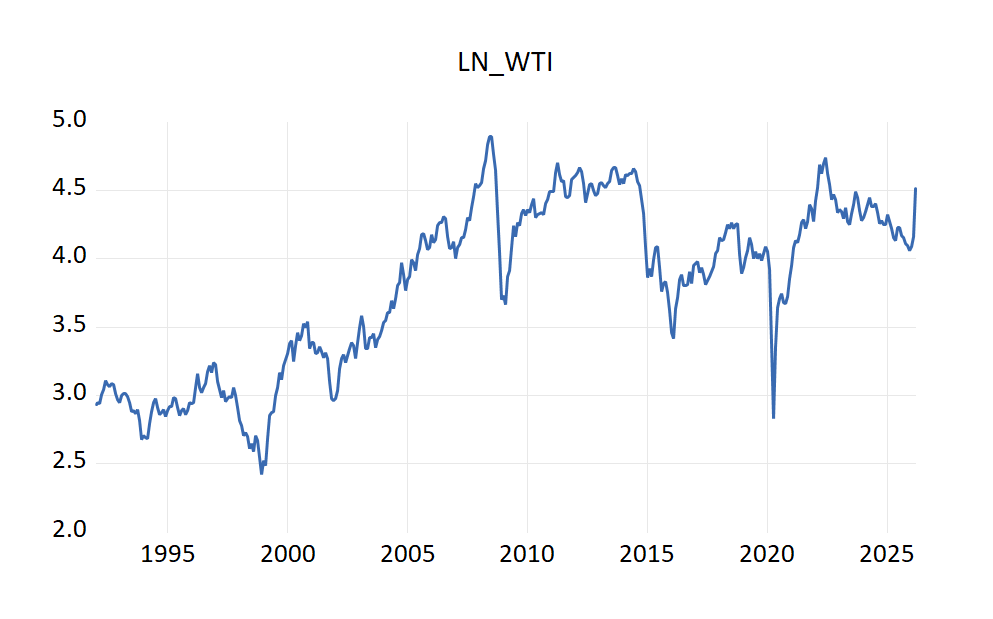
\includegraphics[width=\linewidth]{序列ln_wti时序图.png}
\end{minipage}
\hfill
\begin{minipage}{0.48\textwidth}
\centering
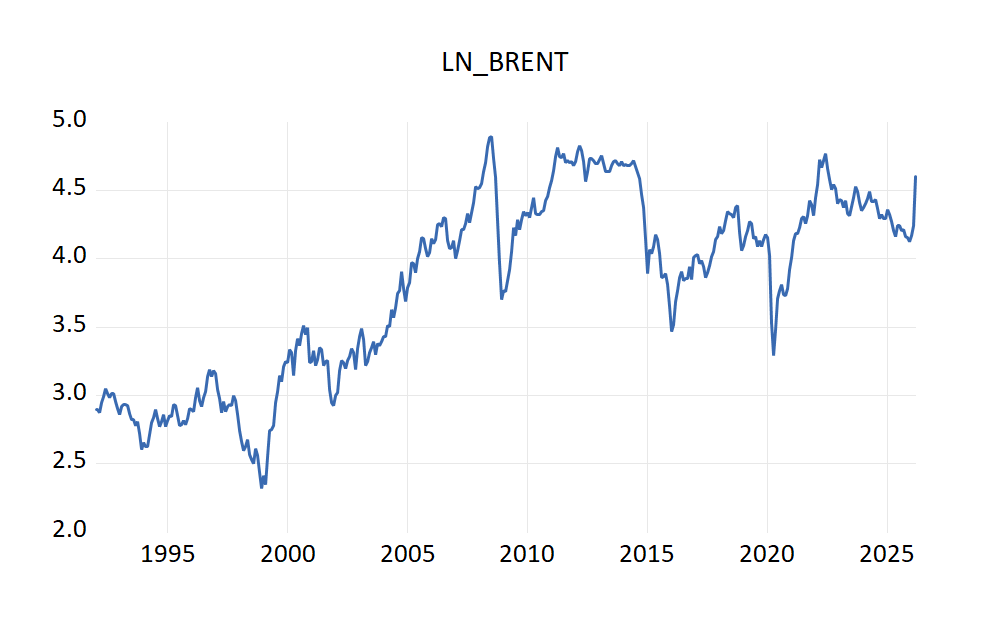
\includegraphics[width=\linewidth]{序列LN_BRENT时序图.png}
\end{minipage}

\vspace{1em} % 上下行间距
% 第二行
\begin{minipage}{0.48\textwidth}
\centering
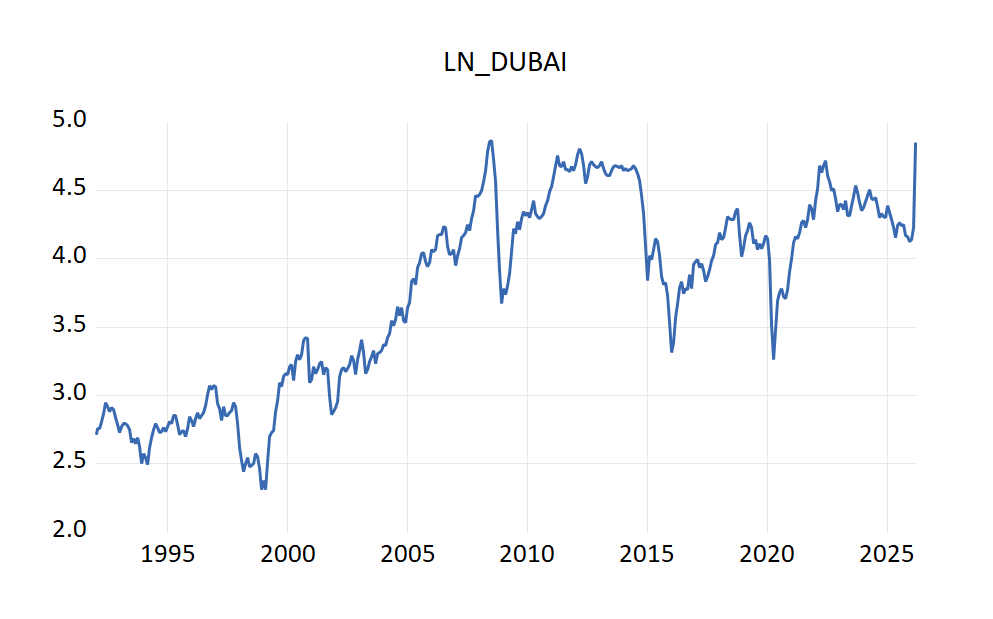
\includegraphics[width=\linewidth]{序列ln_dubai时序图.png}
\end{minipage}

\caption{三大原油价格对数序列时序图}
\label{fig:对数序列时序图}
\end{figure}


\newpage
\section{三大原油价格的对数时间序列建模}


\subsection{序列平稳性检验}

\subsubsection{单位根检验}

三个原始对数价格序列LN\_WTI、LN\_BRENT、LN\_DUBAI的ADF检验结果如表~\ref{tab:adf_level}所示。

\begin{table}[H]
\centering
\caption{三大原油价格对数序列ADF检验p值}
\label{tab:adf_level}
\begin{tabular}{lccc}
\toprule[1.2pt]
检验设定 & LN\_WTI & LN\_BRENT & LN\_DUBAI \\
\midrule[0.75pt]
None & 0.7828 & 0.8150 & 0.8489 \\
Constant & 0.1057 & 0.4108 & 0.4904 \\
Constant, Linear Trend & 0.2747 & 0.1999 & 0.1390 \\
\bottomrule[1.2pt]
\end{tabular}
\end{table}

由表~\ref{tab:adf_level}可知，三种检验设定下，各对数序列的p值均大于0.05，无法拒绝存在单位根的原假设，表明三个对数序列均为非平稳序列。
分别对各对数序列进行一阶差分得到序列
\begin{align}
&\mathrm{DF}\_\mathrm{LN}\_\mathrm{WTI}=\mathrm{LN}\_\mathrm{WTI}_t-\mathrm{LN}\_\mathrm{WTI}_{t-1},
\\
&\mathrm{DF}\_\mathrm{LN}\_\mathrm{BRENT}=\mathrm{LN}\_\mathrm{BRENT}_t-\mathrm{LN}\_\mathrm{BRENT}_{t-1},
\\
&\mathrm{DF}\_\mathrm{LN}\_\mathrm{DUBAI}=\mathrm{LN}\_\mathrm{DUBAI}_t-\mathrm{LN}\_\mathrm{DUBAI}_{t-1},
\end{align}
其时序图如图\ref{fig:df}所示。

\begin{figure}[H]
\centering
% 第一行
\begin{minipage}{0.48\textwidth}
\centering
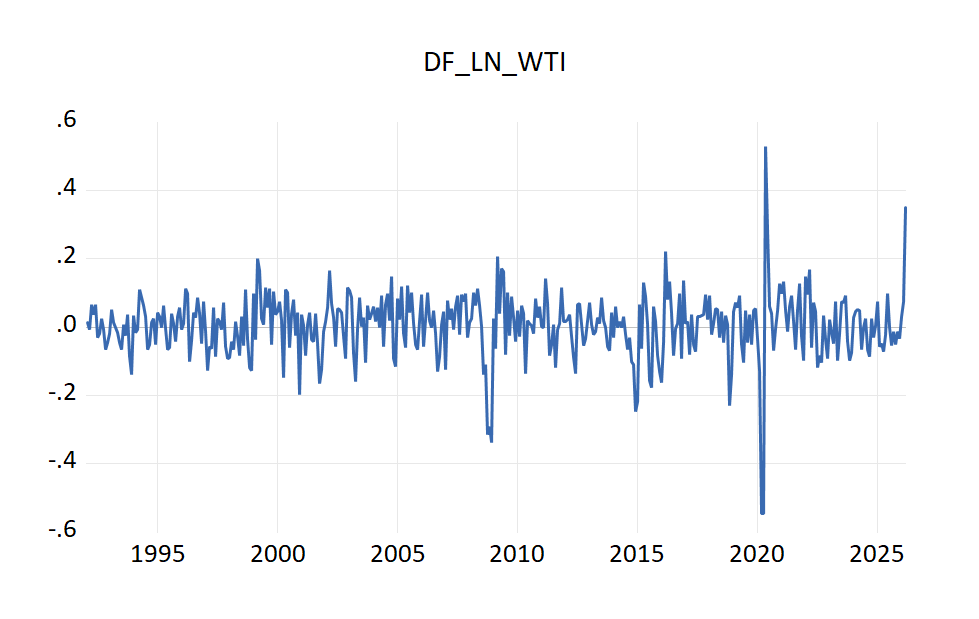
\includegraphics[width=\linewidth]{序列df_ln_wti时序图.png}
\end{minipage}
\hfill
\begin{minipage}{0.48\textwidth}
\centering
\includegraphics[width=\linewidth]{序列DF_LN_BRENT时序图.png}
\end{minipage}

\vspace{1em} % 上下行间距
% 第二行
\begin{minipage}{0.48\textwidth}
\centering
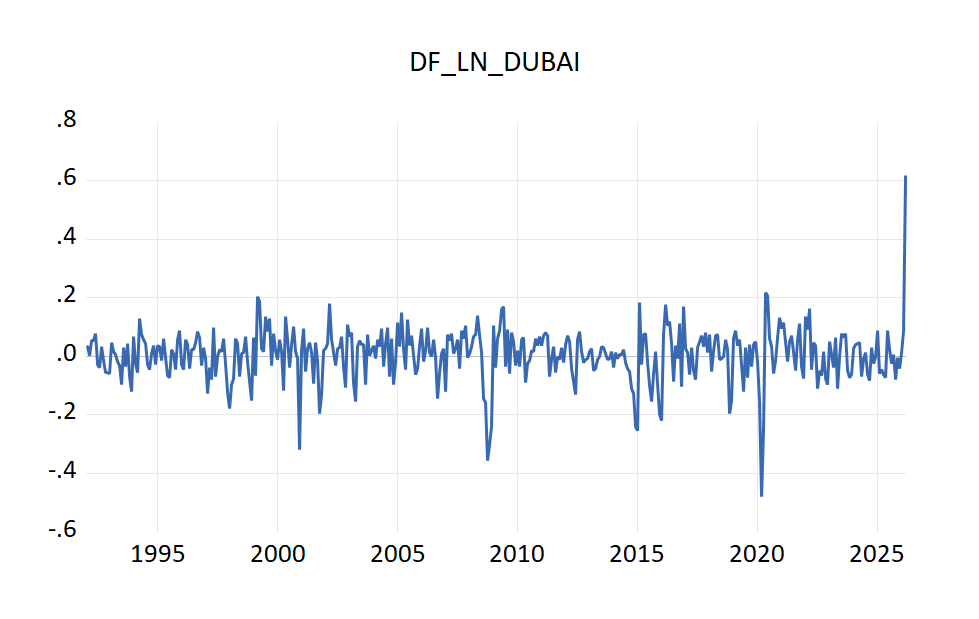
\includegraphics[width=\linewidth]{序列df_ln_dubai时序图.png}
\end{minipage}

\caption{三大原油价格对数一阶差分序列时序图}
\label{fig:df}
\end{figure}

再对各差分序列进行ADF检验，结果分别见表~\ref{table:序列DF_LN_WTI单位根检验不同情形的信息准则对比}、表~\ref{table:序列DF_LN_BRENT的ADF检验不同情形的信息准则对比}、表~\ref{table:序列DF_LN_DUBAI的ADF检验不同情形的信息准则对比}。

\begin{table}[H]
\centering
\caption{序列DF\_LN\_WTI的ADF检验不同情形的信息准则对比}
\label{table:序列DF_LN_WTI单位根检验不同情形的信息准则对比}
\begin{tabular}{lcccc}
\toprule[1.2pt] % 顶部粗线
检验设定 & p值 & AIC准则 & SC准则 & HQ准则 \\
\midrule[0.75pt] % 中间细线
None & 0.0000 & $\mathbf{-1.945408}$ & $\mathbf{-1.935594}$& $\mathbf{-1.941525}$ \\
Constant & 0.0000 & -1.941631 & -1.922005 & -1.933866 \\
Constant,Linear Trend & 0.0000 & -1.936742 & -1.907302 & -1.925093 \\
\bottomrule[1.2pt] % 底部粗线
\end{tabular}
\end{table}

\begin{table}[H]
\centering
\caption{序列DF\_LN\_BRENT的ADF检验不同情形的信息准则对比}
\label{table:序列DF_LN_BRENT的ADF检验不同情形的信息准则对比}
\begin{tabular}{lcccc}
\toprule[1.2pt] % 顶部粗线
检验情形 & p值 &  AIC准则 & SC准则 & HQ准则 \\
\midrule[0.75pt] % 中间细线
None & 0.0000 & $\mathbf{-2.098702}$ & $\mathbf{-2.088888}$ & $\mathbf{-2.094819}$ \\
Constant & 0.0000 & -2.0953098 & -2.075682 & -2.087544 \\
Constant,Linear Trend & 0.0000 & -2.090420 & -2.060979 & -2.078771 \\
\bottomrule[1.2pt] % 底部粗线
\end{tabular}
\end{table}

\begin{table}[H]
\centering
\caption{序列DF\_LN\_DUBAI的ADF检验不同情形的信息准则对比}
\label{table:序列DF_LN_DUBAI的ADF检验不同情形的信息准则对比}
\begin{tabular}{lcccc}
\toprule[1.2pt]
检验情形 & p值 & AIC准则 & SC准则 & HQ准则 \\
\midrule[0.75pt]
None & 0.0000 & \textbf{-2.076381} & \textbf{-2.066567} & \textbf{-2.072498} \\
Constant & 0.0000 & -2.073570 & -2.053943 & -2.065804 \\
Constant,Linear Trend & 0.0000 & -2.068842 & -2.039402 & -2.057194 \\
\bottomrule[1.2pt]
\end{tabular}
\end{table}

由表\ref{table:序列DF_LN_WTI单位根检验不同情形的信息准则对比}、表~\ref{table:序列DF_LN_BRENT的ADF检验不同情形的信息准则对比}、表~\ref{table:序列DF_LN_DUBAI的ADF检验不同情形的信息准则对比}可知，
所有p值均为0.0000<0.05，故三个序列均平稳。根据信息准则，三个序列均选择“\textbf{无截距、无时间趋势}”形式进行建模。


\subsubsection{自相关与偏自相关函数分析}

三个差分序列的ACF和PACF检验分别见图~\ref{fig:序列DF_LN_WTI的ACF和PACF相关图}、图~\ref{fig:序列DF_LN_BRENT的ACF和PACF相关图}、图~\ref{fig:序列DF_LN_DUBAI的ACF和PACF相关图}。

% \begin{figure}[H]
% \centering
% % 第一行
% \begin{minipage}{0.48\textwidth}
% \centering
% 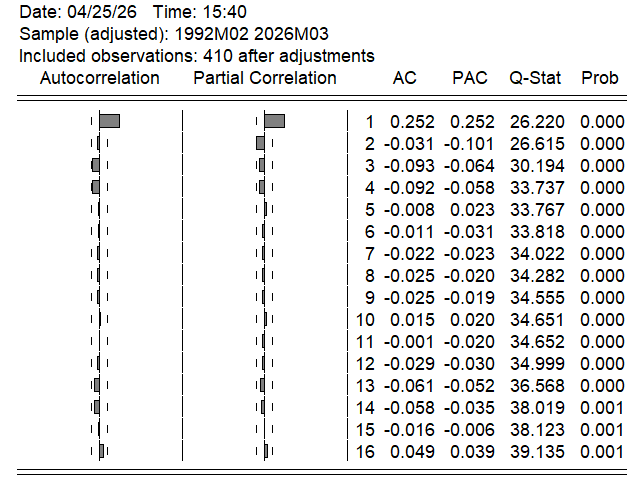
\includegraphics[width=\linewidth]{序列DF_LN_WTI的ACF和PACF相关图.png}
% \end{minipage}
% \hfill
% \begin{minipage}{0.48\textwidth}
% \centering
% 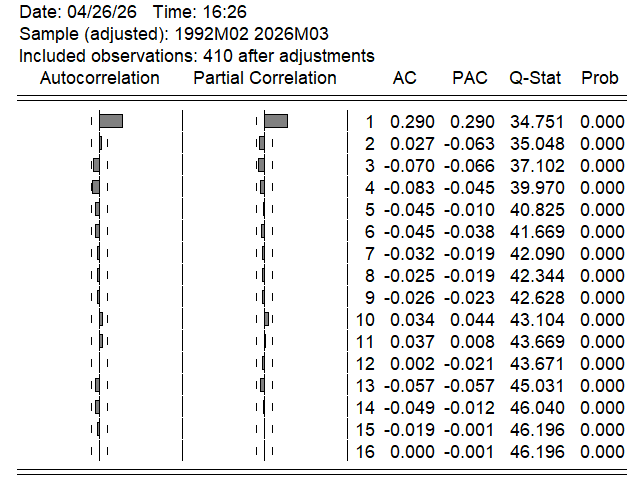
\includegraphics[width=\linewidth]{序列DF_LN_DUBAI的ACF和PACF相关图.png}
% \end{minipage}

% \vspace{1em} % 上下行间距
% % 第二行
% \begin{minipage}{0.48\textwidth}
% \centering
% 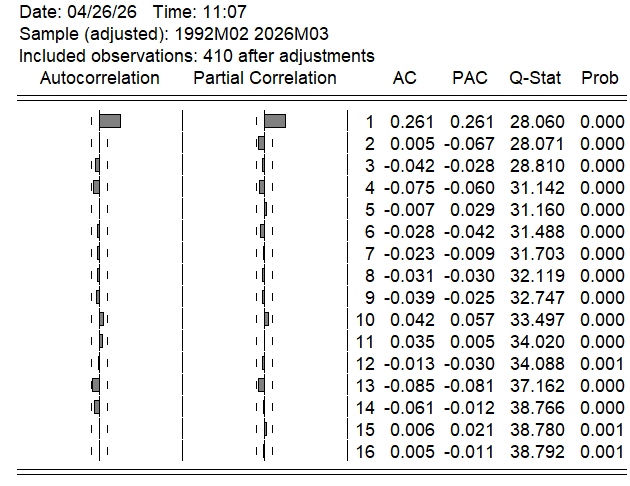
\includegraphics[width=\linewidth]{序列DF_LN_BRENT的ACF和PACF相关图.png}
% \end{minipage}

% \caption{三大原油价格对数一阶差分序列的ACF和PACF图}
% \label{fig:ACF-PACF}
% \end{figure}

\begin{figure}[H]
\centering
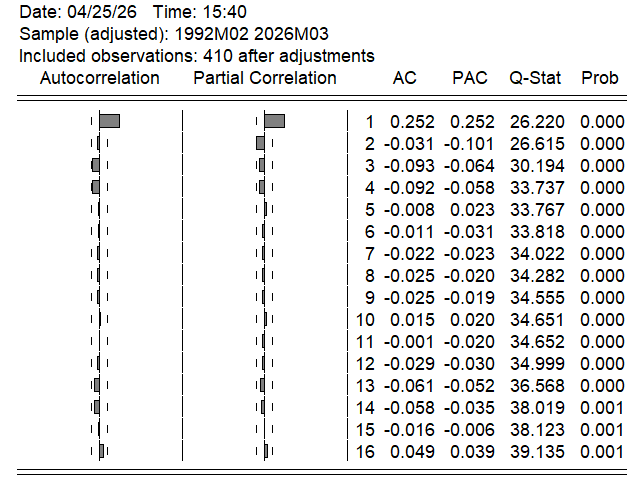
\includegraphics[width=0.8\textwidth]{序列DF_LN_WTI的ACF和PACF相关图.png}
\caption{序列DF\_LN\_WTI的ACF和PACF相关图}
\label{fig:序列DF_LN_WTI的ACF和PACF相关图}
\end{figure}

\begin{figure}[H]
\centering
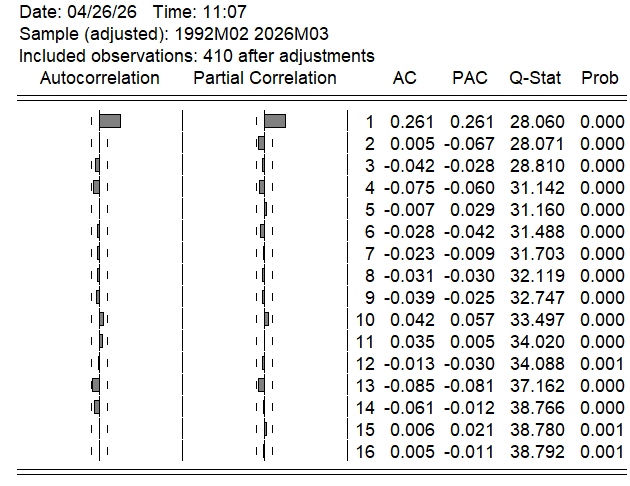
\includegraphics[width=0.8\textwidth]{序列DF_LN_BRENT的ACF和PACF相关图.png}
\caption{序列DF\_LN\_BRENT的ACF和PACF相关图}
\label{fig:序列DF_LN_BRENT的ACF和PACF相关图}
\end{figure}

\begin{figure}[H]
\centering
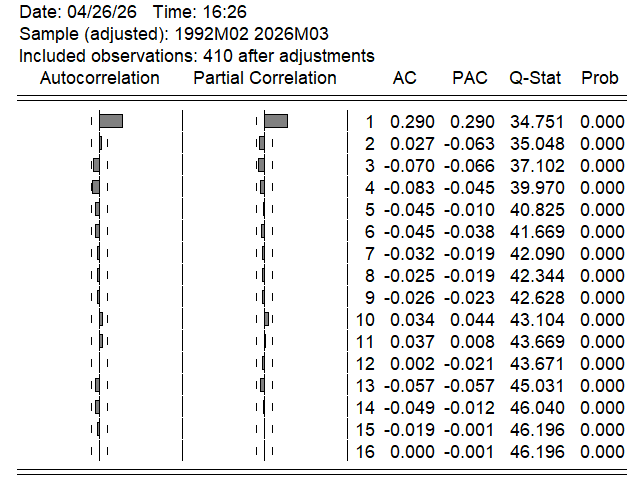
\includegraphics[width=0.8\textwidth]{序列DF_LN_DUBAI的ACF和PACF相关图.png}
\caption{序列DF\_LN\_DUBAI的ACF和PACF相关图}
\label{fig:序列DF_LN_DUBAI的ACF和PACF相关图}
\end{figure}

由图~\ref{fig:序列DF_LN_WTI的ACF和PACF相关图}、图~\ref{fig:序列DF_LN_BRENT的ACF和PACF相关图}、图~\ref{fig:序列DF_LN_DUBAI的ACF和PACF相关图}可知，DF\_LN\_WTI的ACF 1阶截尾、PACF 2阶截尾；DF\_LN\_BRENT和DF\_LN\_DUBAI的ACF和PACF均为1阶截尾。并且三个序列各滞后阶数的Q统计量p值均小于0.05，拒绝白噪声原假设，具备建模基础。

\subsection{均值模型的构建与检验}

\subsubsection{均值模型的构建与优选}

根据每个序列自相关(ACF)与偏自相关函数(PACF)的特征，对每个序列分别拟合AR、MA、ARMA系列低阶模型，并将各个序列的不同模型的系数显著性检验结果和AIC/SC/HQ值分别汇总到如下表~\ref{tab:arma_combined}、表~\ref{tab:arma_pvalue_brent}、表~\ref{tab:arma_pvalue_dubai}中。

\begin{table}[H]
\centering
\caption{序列DF\_LN\_WTI的ARMA模型系数显著性检验与信息准则对比结果}
\label{tab:arma_combined}
\setlength{\tabcolsep}{4pt}  % 适当缩小列间距以适应页面
\begin{tabular}{cccccc ccc}
\toprule[1.2pt]
\multirow{2}{*}{模型} & \multicolumn{4}{c}{系数显著性（p值）} & \multicolumn{3}{c}{信息准则} \\
\cmidrule(lr){2-5} \cmidrule(lr){6-8}
& AR(1) & AR(2) & MA(1) & MA(2) & AIC & SC & HQ \\
\midrule[0.75pt]
ARMA(1,1)  & 0.9472 & --    & 0.0313 & --    & -1.9453 & -1.9159 & -1.9336 \\
ARMA(2,2)  & 0.0000 & 0.2580 & 0.0000 & 0.2630 & -1.9492 & -1.9002 & -1.9298 \\
ARMA(2,1)  & \textbf{0.0000} & \textbf{0.0000} & \textbf{0.0001} & --    & -1.9502 & -1.9109 & -1.9347 \\
ARMA(1,2)  & \textbf{0.0000} & --    & \textbf{0.0000} & \textbf{0.0000} & -1.9521 & -1.9130 & -1.9366 \\
AR(1)      & \textbf{0.0000} & --    & --    & --    & -1.9428 & -1.9232 & -1.9350 \\
AR(2)      & \textbf{0.0000} & \textbf{0.0174} & --    & --    & -1.9483 & -1.9189 & -1.9367 \\
MA(1)      & --    & --    & \textbf{0.0000} & --    & \textbf{-1.9501} & \textbf{-1.9305} & \textbf{-1.9424} \\
MA(2)      & --    & --    & 0.0000 & 0.9260 & -1.9453 & -1.9159 & -1.9336 \\
\bottomrule[1.2pt]
\end{tabular}
\end{table}

\begin{table}[H]
\centering
\caption{序列DF\_LN\_BRENT的ARMA模型系数显著性检验和信息准则对比图}
\label{tab:arma_pvalue_brent}
\setlength{\tabcolsep}{4pt}  % 适当缩小列间距以适应页面
\begin{tabular}{cccccc ccc}
\toprule[1.2pt]
\multirow{2}{*}{模型} & \multicolumn{4}{c}{系数显著性（p值）} & \multicolumn{3}{c}{信息准则} \\
\cmidrule(lr){2-5} \cmidrule(lr){6-8}
& AR(1) & AR(2) & MA(1) & MA(2) & AIC & SC & HQ \\
\midrule[0.75pt]
ARMA(1,1)  & 0.6565 & - & 0.1044 & - & -2.0954 & -2.0660 & -2.0837 \\
ARMA(2,2)  & 0.0000 & 0.2551 & 0.0000 & 0.3959 & -2.0928 & -2.0438 & -2.0734 \\
ARMA(2,1)  & \textbf{0.0000} & \textbf{0.0000} & \textbf{0.0000} & -  & -2.0963 & -2.0571 & -2.0808 \\
ARMA(1,2)  & 0.9917 & - & 0.9190 & 0.9894 & -2.0905 & -2.0513 & -2.0750 \\
AR(1)      & \textbf{0.0000} & - & - & - & -2.0961 & -2.0765 & -2.0883 \\
AR(2)      & 0.0000 & 0.0953 & - & - & -2.0959 & -2.0665 & -2.0843 \\
MA(1)      & - & - & \textbf{0.0000} & - & \textbf{-2.1000} & \textbf{-2.0804} & \textbf{-2.0922} \\
MA(2)      & - & - & 0.0000 & 0.6528 & -2.0954 & -2.0660 & -2.0837 \\
\bottomrule[1.2pt]
\end{tabular}
\end{table}

\begin{table}[H]
\centering
\caption{序列DF\_LN\_DUBAI的ARMA模型系数显著性检验和信息准则对比图}
\label{tab:arma_pvalue_dubai}
\setlength{\tabcolsep}{4pt}  % 适当缩小列间距以适应页面
\begin{tabular}{cccccc ccc}
\toprule[1.2pt]
\multirow{2}{*}{模型} & \multicolumn{4}{c}{系数显著性（p值）} & \multicolumn{3}{c}{信息准则} \\
\cmidrule(lr){2-5} \cmidrule(lr){6-8}
& AR(1) & AR(2) & MA(1) & MA(2) & AIC & SC & HQ \\
\midrule[0.75pt]
ARMA(1,1) & 0.1009 & - & 0.1818 & - & -2.0722 & -2.0428 & -2.0605 \\
ARMA(2,2) & 0.0000 & 0.0388 & 0.0000 & 0.6405 & -2.0729 & -2.0239 & -2.0535 \\
ARMA(2,1) & \textbf{0.0000} & \textbf{0.0000} & \textbf{0.0000} & - & -2.0771 & -2.0379 & -2.0616 \\
ARMA(1,2) & 0.8909 & - & 0.5020 & 0.6261 & -2.0686 & -2.0294 & -2.0531 \\
AR(1) & \textbf{0.0000} & - & - & - & \textbf{-2.0733} & \textbf{-2.0537} & \textbf{-2.0656} \\
AR(2) & 0.0000 & 0.0769 & - & - & -2.0737 & -2.0443 & -2.0621 \\
MA(1) & - & - & \textbf{0.0000} & - & -2.0732 & -2.0537 & -2.0655 \\
MA(2) & - & - & \textbf{0.0000} & \textbf{0.0418} & -2.0733 & -2.0440 & -2.0617 \\
\bottomrule[1.2pt]
\end{tabular}
\end{table}

根据系数显著性（p<0.05）和AIC/SC/HQ信息准则，将各序列的最优均值模型汇总于表~\ref{tab:best_arma_all}中。

\begin{table}[H]
\centering
\caption{三大原油价格序列最优ARMA均值模型}
\label{tab:best_arma_all}
\begin{tabular}{lcccc}
\toprule
序列 & 最优模型 & 模型系数 & 标准误差 & p值 \\
\midrule
DF\_LN\_WTI   & MA(1) & 0.2272 & 0.0542 & 0.0000 \\
DF\_LN\_BRENT & MA(1) & 0.2861 & 0.0409 & 0.0000 \\
DF\_LN\_DUBAI & AR(1) & 0.3283 & 0.0348 & 0.0000 \\
\bottomrule
\end{tabular}
\end{table}


\subsubsection{模型适应性检验}

对表~\ref{tab:best_arma_all}中三个最优均值模型的残差序列进行Q检验，结果分别如图~\ref{fig:序列DF_LN_WTI的MA(1)模型的适应性检验结果图}、图~\ref{fig:序列DF_LN_BRENT的MA(1)模型适应性检验图}、图~\ref{fig:序列DF_LN_DUBAI的AR(1)模型适应性检验图}所示。

% \begin{figure}[H]
% \centering
% % 第一行
% \begin{minipage}{0.48\textwidth}
% \centering
% 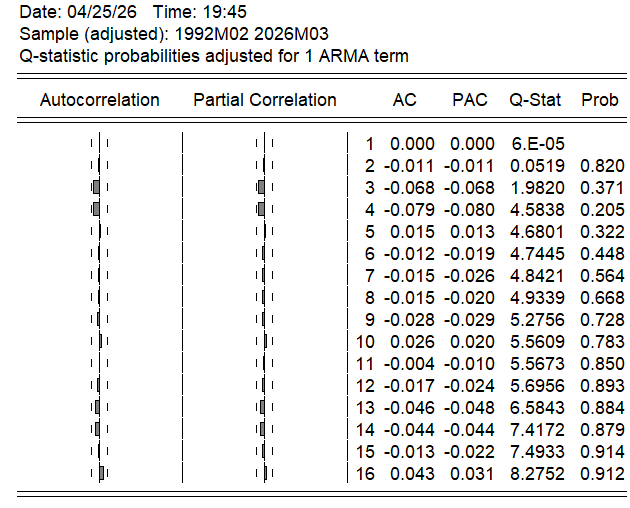
\includegraphics[width=\linewidth]{序列DF_LN_WTI的MA(1)模型的适应性检验结果图.png}
% \end{minipage}
% \hfill
% \begin{minipage}{0.48\textwidth}
% \centering
% 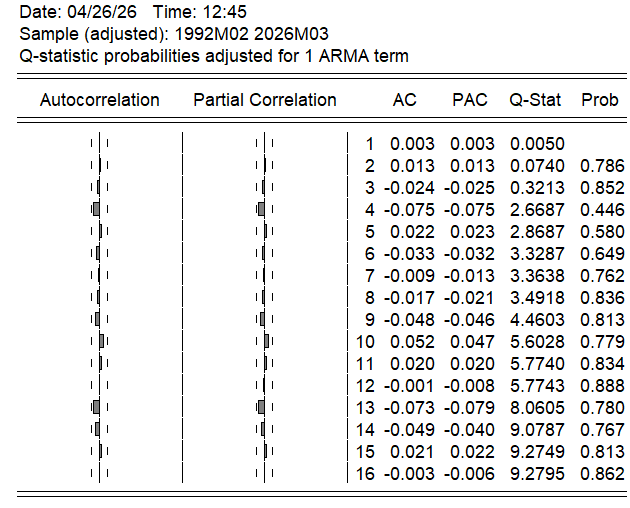
\includegraphics[width=\linewidth]{序列DF_LN_BRENT的MA(1)模型适应性检验图.png}
% \end{minipage}

% \vspace{1em} % 上下行间距
% % 第二行
% \begin{minipage}{0.48\textwidth}
% \centering
% 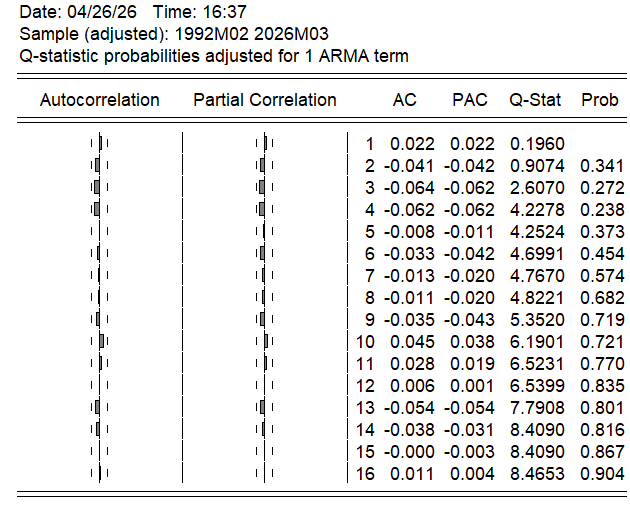
\includegraphics[width=\linewidth]{序列DF_LN_DUBAI的AR(1)模型适应性检验图.png}
% \end{minipage}

% \caption{三大原油价格最优均值模型适应性检验图}
% \label{fig:模型适应性检验}
% \end{figure}

\begin{figure}[H]
\centering
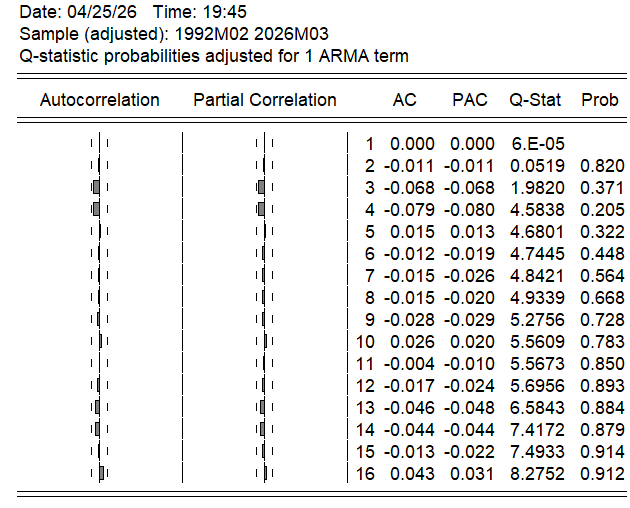
\includegraphics[width=0.8\textwidth]{序列DF_LN_WTI的MA(1)模型的适应性检验结果图.png}
\caption{序列DF\_LN\_WTI的MA(1)模型的适应性检验结果图}
\label{fig:序列DF_LN_WTI的MA(1)模型的适应性检验结果图}
\end{figure}

\begin{figure}[H]
\centering
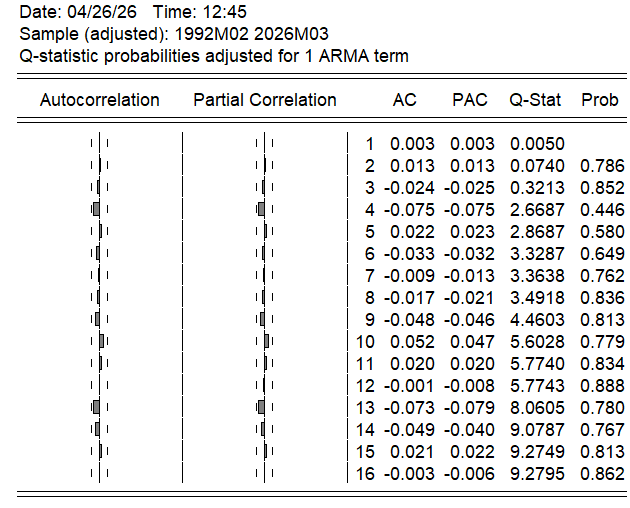
\includegraphics[width=0.8\textwidth]{序列DF_LN_BRENT的MA(1)模型适应性检验图.png}
\caption{序列DF\_LN\_BRENT的MA(1)模型适应性检验图}
\label{fig:序列DF_LN_BRENT的MA(1)模型适应性检验图}
\end{figure}

\begin{figure}[H]
\centering
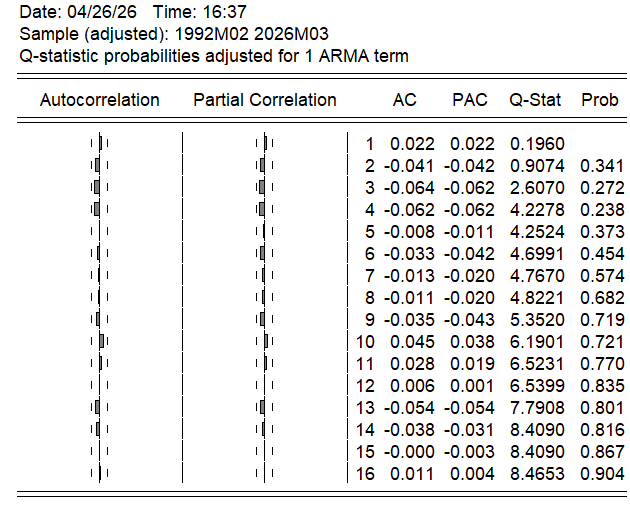
\includegraphics[width=0.8\textwidth]{序列DF_LN_DUBAI的AR(1)模型适应性检验图.png}
\caption{序列DF\_LN\_DUBAI的AR(1)模型适应性检验图}
\label{fig:序列DF_LN_DUBAI的AR(1)模型适应性检验图}
\end{figure}

由图~\ref{fig:序列DF_LN_WTI的MA(1)模型的适应性检验结果图}、图~\ref{fig:序列DF_LN_BRENT的MA(1)模型适应性检验图}、图~\ref{fig:序列DF_LN_DUBAI的AR(1)模型适应性检验图}可知，三个序列各滞后阶数的Q统计量的p值均大于0.05，残差为白噪声，说明模型的均值信息提取充分。

\subsubsection{条件异方差检验}

考虑到条件异方差多表现为短期波动聚集，低阶滞后项已能捕捉绝大多数 ARCH 效应；同时，滞后阶数过高会导致检验自由度下降、估计偏差增大，故本文只选取滞后 4、5、6 阶进行 ARCH-LM 检验。
对三个最优均值模型的残差进行ARCH-LM检验，结果见表~\ref{tab:ARCH-LM1}。

\begin{table}[H]
\centering
\caption{ARCH-LM检验结果}
\label{tab:ARCH-LM1}
\setlength{\tabcolsep}{4pt}  % 适当缩小列间距以适应页面
\begin{tabular}{lcccc ccc}
\toprule[1.2pt]
\multirow{2}{*}{$\quad\quad\,$序列(模型)} & \multicolumn{3}{c}{F统计量p值}  \\
\cmidrule(lr){2-4}
& 滞后4阶 & 滞后5阶 & 滞后6阶 \\
\midrule[0.75pt]
DF\_LN\_WTI(MA(1))   & 0.0000 & 0.0000  & 0.0000  \\
DF\_LN\_BRENT(MA(1)) & 0.0010 & 0.0025  & 0.0056  \\
DF\_LN\_DUBAI(AR(1)) & 0.0048 & 0.0108  & 0.0214  \\
\bottomrule
\end{tabular}
\end{table}

由表~\ref{tab:ARCH-LM1}可知，所有序列各滞后阶数的F统计量p值均小于0.05，均存在显著的条件异方差。

再对三个最优均值模型的残差平方序列进行Q检验，结果分别如图~\ref{fig:序列DF_LN_WTI的MA(1)模型残差的平方的Q检验结果图}、图~\ref{fig:序列DF_LN_BRENT的MA(1)模型条件异方差检验图4}、图~\ref{fig:序列DF_LN_DUBAI的AR(1)模型条件异方差检验图4}所示。

\begin{figure}[H]
\centering
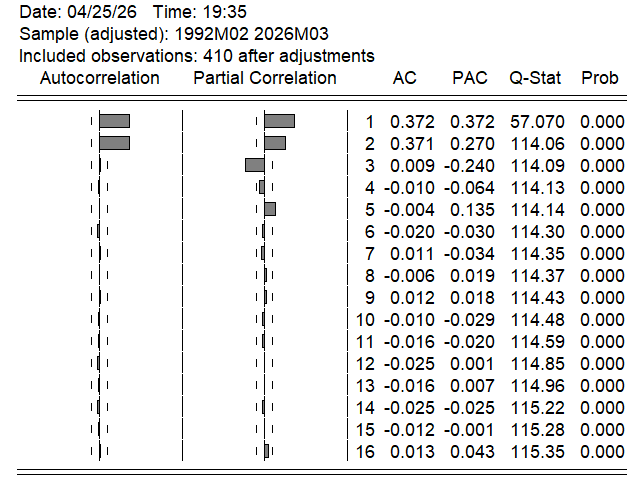
\includegraphics[width=0.8\textwidth]{序列DF_LN_WTI的MA(1)模型残差的平方的Q检验结果图.png}
\caption{序列DF\_LN\_WTI的MA(1)模型残差的平方的Q检验结果图}
\label{fig:序列DF_LN_WTI的MA(1)模型残差的平方的Q检验结果图}
\end{figure}

\begin{figure}[H]
\centering
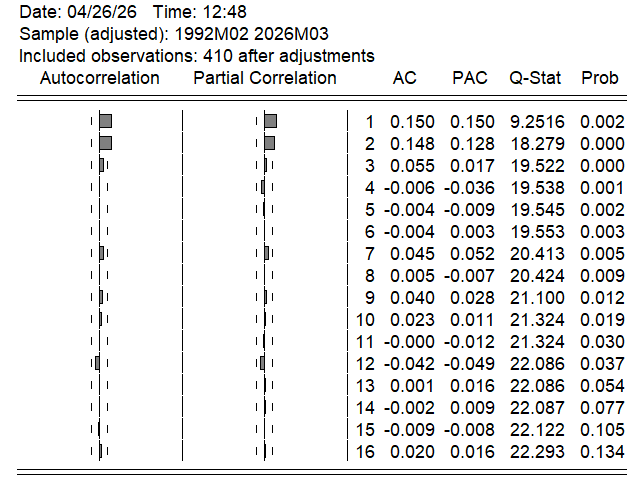
\includegraphics[width=0.8\textwidth]{序列DF_LN_BRENT的MA(1)模型条件异方差检验图4.png}
\caption{序列DF\_LN\_BRENT的AR(1)模型残差平方序列的Q检验图}
\label{fig:序列DF_LN_BRENT的MA(1)模型条件异方差检验图4}
\end{figure}

\begin{figure}[H]
\centering
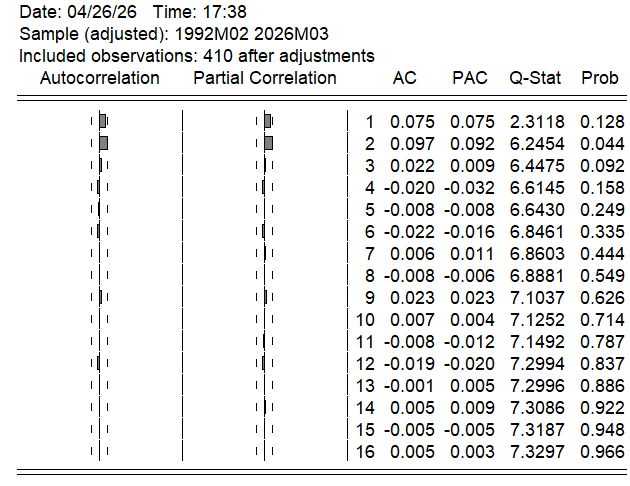
\includegraphics[width=0.8\textwidth]{序列DF_LN_DUBAI的AR(1)模型条件异方差检验图4.png}
\caption{序列DF\_LN\_DUBAI的AR(1)模型残差平方序列的Q检验图}
\label{fig:序列DF_LN_DUBAI的AR(1)模型条件异方差检验图4}
\end{figure}

由图~\ref{fig:序列DF_LN_WTI的MA(1)模型残差的平方的Q检验结果图}、图~\ref{fig:序列DF_LN_BRENT的MA(1)模型条件异方差检验图4}、图~\ref{fig:序列DF_LN_DUBAI的AR(1)模型条件异方差检验图4}可知
\begin{itemize}
\item 序列DF\_LN\_WTI的MA(1)模型残差平方各阶Q统计量p值均为0.000<0.05，存在极显著的条件异方差；

\item 序列DF\_LN\_BRENT的AR(1)模型残差平方在前12阶Q统计量p值均<0.05，条件异方差效应显著；

\item 序列DF\_LN\_DUBAI的的AR(1)模型残差平方在滞后2阶的Q统计量p值为0.044<0.05，虽然后续滞后阶数p值逐渐增大，但仍表明存在微弱但统计显著的条件异方差。
\end{itemize}

综上，这三个序列的最优均值模型均存在显著的条件异方差。为此，进一步构建GARCH族模型，以同时刻画序列的均值过程与异方差特征。



\subsection{GARCH族模型构建与检验}

各序列的直方图与描述性统计如图~\ref{fig:序列DF_LN_WTI的直方图与描述性统计图}、图~\ref{fig:序列DF_LN_BRENT的直方图与描述性统计图}、图~\ref{fig:序列DF_LN_DUBAI的直方图与描述性统计图}所示。

\begin{figure}[H]
\centering
\includegraphics[width=0.8\textwidth]{序列DF_LN_WTI的直方图与描述性统计图.png}
\caption{序列DF\_LN\_WTI的直方图与描述性统计}
\label{fig:序列DF_LN_WTI的直方图与描述性统计图}
\end{figure}

\begin{figure}[H]
\centering
\includegraphics[width=0.8\textwidth]{序列DF_LN_BRENT的直方图与描述性统计图.png}
\caption{序列DF\_LN\_BRENT的直方图与描述性统计}
\label{fig:序列DF_LN_BRENT的直方图与描述性统计图}
\end{figure}

\begin{figure}[H]
\centering
\includegraphics[width=0.8\textwidth]{序列DF_LN_DUBAI的直方图与描述性统计图.png}
\caption{序列DF\_LN\_DUBAI的直方图与描述性统计}
\label{fig:序列DF_LN_DUBAI的直方图与描述性统计图}
\end{figure}

图~\ref{fig:序列DF_LN_WTI的直方图与描述性统计图}、图~\ref{fig:序列DF_LN_BRENT的直方图与描述性统计图}、图~\ref{fig:序列DF_LN_DUBAI的直方图与描述性统计图}显示序列DF\_LN\_WTI、DF\_LN\_BRENT、DF \_ LN\_DUBAI的峰度分别为10.85、9.02、8.76，显著大于正态分布的峰度3，且Jarque-Bera正态性检验p值均为0.0000<0.05，拒绝序列服从正态分布的原假设，具有典型的\textbf{尖峰厚尾}特征。传统GARCH模型的正态分布假设难以刻画金融时间序列的厚尾性，而t分布能够更好地拟合极端波动的尾部风险。故后续所有GARCH族模型均采用Student's $t$分布。

\subsubsection{GARCH族模型构建与优选}

\subsubsubsection{WTI原油价格}\hspace{0pt}\par

\vspace{6pt}

对序列DF\_LN\_WTI，在MA(1)均值方程基础上，构建MA(1)-GARCH、MA(1)-TARCH、MA(1)-EGARCH系列低阶模型，并将各模型的系数显著性检验结果和信息准则值分别汇总到表~\ref{tab:wti_garch_p}和表~\ref{tab:wti_garch_criteria}中。

\begin{table}[H]
\centering
\caption{DF\_LN\_WTI序列GARCH族模型系数显著性检验结果}
\label{tab:wti_garch_p}
\setlength{\tabcolsep}{4pt}  % 适当缩小列间距以适应页面
\begin{tabular}{lccccc}
\toprule[1.2pt]
\multirow{2}{*}{$\quad\quad\,\,\,\,\,$模型名称} & \multicolumn{4}{c}{系数显著性(p值)}  \\
\cmidrule(lr){2-5}
& 常数项C & ARCH项 & 非对称项 & GARCH项 \\
\midrule[0.75pt]
MA(1)-GARCH(1,0)-t     & \textbf{0.0000} & \textbf{0.0033} & - & - \\
MA(1)-GARCH(2,0)-t     & 0.0000 & 0.0400/0.0504 & - & - \\
MA(1)-GARCH(1,1)-t     & \textbf{0.0292} & \textbf{0.0075} & - & \textbf{0.0002} \\
MA(1)-GARCH(1,2)-t     & 0.0514 & 0.0280 & - & 0.2649/0.9921 \\
MA(1)-GARCH(2,1)-t     & \textbf{0.0617} & \textbf{0.0046}/\textbf{0.0042} & - & \textbf{0.0000} \\
MA(1)-GARCH(2,2)-t     & 0.1663/0.0122 & 0.0116 & - & 0.0000/0.0211 \\
\midrule
MA(1)-TARCH(1,0)-t     & 0.0000 & 0.7631 & 0.0012 & - \\
MA(1)-TARCH(2,0)-t     & 0.0000 & 0.7519/0.1519 & 0.0017 & - \\
MA(1)-TARCH(1,1)-t     & 0.0000 & 0.8927 & 0.0014 & 0.7877 \\
MA(1)-TARCH(1,2)-t     & 0.0000 & 0.9659 & 0.0004 & 0.0935/0.0513 \\
MA(1)-TARCH(2,1)-t     & 0.0000 & 0.9134/0.1907 & 0.0012 & 0.5160 \\
MA(1)-TARCH(2,2)-t     & 0.0000 & 0.8634/0.3143 & 0.0011 & 0.3208/0.4738 \\
\midrule
MA(1)-EGARCH(1,0)-t    & 0.0000 & 0.0625 & 0.0016 & - \\
MA(1)-EGARCH(2,0)-t    & 0.0000 & 0.1981/0.0000 & 0.0020 & - \\
MA(1)-EGARCH(1,1)-t    & \textbf{0.0113} & \textbf{0.0158} & \textbf{0.0193} & \textbf{0.0000} \\
MA(1)-EGARCH(1,2)-t    & 0.0232 & 0.0381 & 0.0121 & 0.0293/0.0797 \\
MA(1)-EGARCH(2,1)-t    & 0.0001 & 0.1802/0.0042 & 0.0028 & 0.6293 \\
MA(1)-EGARCH(2,2)-t    & 0.0104 & 0.1807/0.0272 & 0.0037 & 0.4647/0.0447 \\
\bottomrule[1.2pt]
\end{tabular}
\end{table}

\begin{table}[H]
\centering
\caption{DF\_LN\_WTI序列GARCH族模型信息准则结果对比}
\label{tab:wti_garch_criteria}
\setlength{\tabcolsep}{4pt}  % 适当缩小列间距以适应页面
\begin{tabular}{lcccc}
\toprule[1.2pt]
\multirow{2}{*}{$\quad\quad\,\,\,\,\,$模型名称} & \multicolumn{1}{c}{p值} & \multicolumn{3}{c}{信息准则} \\
\cmidrule(lr){2-2} \cmidrule(lr){3-5}
& MA(1) & AIC & SC & HQ \\
\midrule[0.75pt]
MA(1)-GARCH(1,0)-t     & 0.0030 & -2.1922  & -2.1531  & -2.1767  \\
MA(1)-GARCH(2,0)-t     & 0.0001 & -2.2011  & -2.1520  & -2.1817  \\
MA(1)-GARCH(1,1)-t     & 0.0008 & -2.2037  & -2.1547  & -2.1843  \\
MA(1)-GARCH(1,2)-t     & 0.0008 & -2.1988  & -2.1400  & -2.1755  \\
MA(1)-GARCH(2,1)-t     & 0.0016 & -2.2082  & -2.1495  & -2.1850  \\
MA(1)-GARCH(2,2)-t     & 0.0005 & -2.2140  & -2.1418  & -2.1832  \\
\midrule
MA(1)-TARCH(1,0)-t     & 0.0000 & -2.2342  & -2.1852  & -2.2148  \\
MA(1)-TARCH(2,0)-t     & 0.0000 & -2.2377  & -2.1789  & -2.2144 \\
MA(1)-TARCH(1,1)-t     & 0.0000 & -2.2296  & -2.1708 & -2.2063  \\
MA(1)-TARCH(1,2)-t     & 0.0000 & -2.2323  & -2.1637  & -2.2052  \\
MA(1)-TARCH(2,1)-t     & 0.0000 & -2.2357  & -2.1671  & -2.2086  \\
MA(1)-TARCH(2,2)-t     & 0.0000 & -2.2332  & -2.1548  & -2.2022  \\
\midrule
MA(1)-EGARCH(1,0)-t    & 0.0000 & -2.1906  & -2.1417  & -2.1713  \\
MA(1)-EGARCH(2,0)-t    & 0.0000 & -2.2231  & -2.1644  & -2.1999  \\
MA(1)-EGARCH(1,1)-t    & 0.0000 & \textbf{-2.2182} & \textbf{-2.1594} & \textbf{-2.1949} \\
MA(1)-EGARCH(1,2)-t    & 0.0000 & -2.2155  & -2.1469  & -2.1883  \\
MA(1)-EGARCH(2,1)-t    & 0.0000 & -2.2187  & -2.1501  & -2.1915  \\
MA(1)-EGARCH(2,2)-t    & 0.0000 & -2.2252  & -2.1468  & -2.1942  \\
\bottomrule
\end{tabular}
\end{table}

由表~\ref{tab:wti_garch_p}和表~\ref{tab:wti_garch_criteria}可知，MA(1)-EGARCH(1,1)-t模型所有参数均显著（p<0.05）且信息准则最优，其结果如图\ref{fig:wti_egarch}所示。

\begin{figure}[H]
\centering
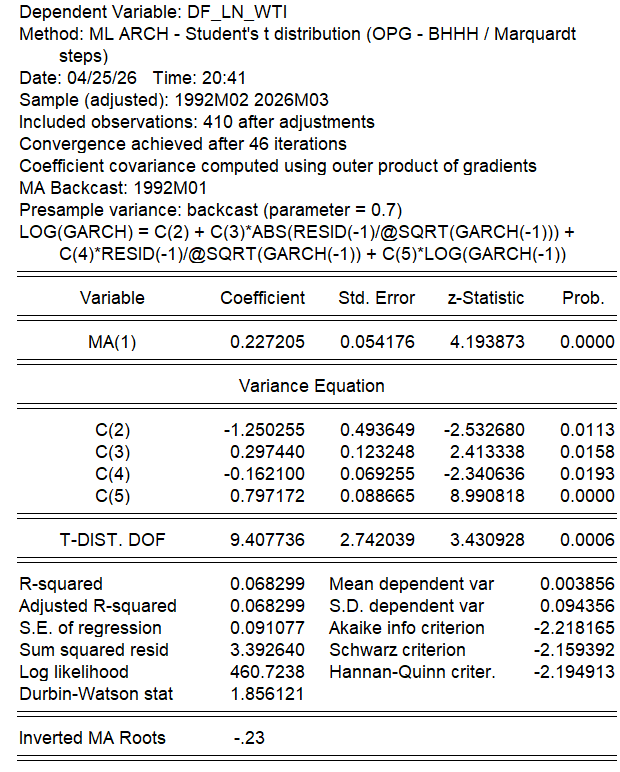
\includegraphics[width=0.7\textwidth]{序列LN_WTI的MA(1)-EGARCH(1,1)模型结果图.png}
\caption{MA(1)-EGARCH(1,1)-t模型估计结果图（WTI）}
\label{fig:wti_egarch}
\end{figure}

由图~\ref{fig:wti_egarch}可知，序列DF\_LN\_WTI的MA(1)-EGARCH(1,1)-t模型的均值方程和方差方程为
\begin{align}\label{eq:序列DF_LN_WTI的MA(1)-EGARCH(1,1)-t模型均值方程}
\mathrm{DF}\_\mathrm{LN}\_\mathrm{WTI}_t=\varepsilon _t+\theta \varepsilon _{t-1}=\varepsilon _t+0.227205\cdot \varepsilon _{t-1},
\end{align}
\begin{gather}\label{eq:序列DF_LN_WTI的MA(1)-EGARCH(1,1)-t模型方差方程}
\begin{aligned}
\ln \left( \sigma _{t}^{2} \right) &=\omega +\alpha \left| \frac{\varepsilon _{t-1}}{\sigma _{t-1}} \right|+\gamma \frac{\varepsilon _{t-1}}{\sigma _{t-1}}+\beta \ln \left( \sigma _{t-1}^{2} \right) 
\\
&=-1.250255+0.297440\cdot \left| \frac{\varepsilon _{t-1}}{\sigma _{t-1}} \right|-0.162100\cdot \frac{\varepsilon _{t-1}}{\sigma _{t-1}}
\\
&\quad +0.797172\cdot \ln \left( \sigma _{t-1}^{2} \right) ,
\end{aligned}
\end{gather}
其中，$\varepsilon_t$ 为扰动项，$\sigma_t^2$ 为条件方差，$\theta$ 为移动平均系数，$\omega$ 为方差方程常数项，$\alpha$ 为ARCH项系数，$\gamma$ 为非对称项系数，$\beta$ 为GARCH项系数，模型扰动项$\varepsilon _t\sim t(9.407736)$。


\subsubsubsection{Brent原油价格}\hspace{0pt}\par

\vspace{6pt}

类似地，对序列DF\_LN\_Brent，在MA(1)均值方程基础上，构建MA(1)-GARCH、MA(1)-TARCH、MA(1)-EGARCH系列低阶模型，并将各模型的系数显著性检验结果和信息准则值分别汇总到表~\ref{tab:brent_garch_p}和表~\ref{tab:brent_garch_criteria}。

\begin{table}[H]
\centering
\caption{DF\_LN\_BRENT序列GARCH族模型系数显著性检验结果}
\label{tab:brent_garch_p}
\setlength{\tabcolsep}{4pt}  % 适当缩小列间距以适应页面
\begin{tabular}{lccccc}
\toprule[1.2pt]
\multirow{2}{*}{$\quad\quad\,\,\,\,\,$模型名称} & \multicolumn{4}{c}{系数显著性(p值)}  \\
\cmidrule(lr){2-5}
& 常数项C & ARCH项 & 非对称项 & GARCH项 \\
\midrule[0.75pt]
MA(1)-GARCH(1,0)-t & \textbf{0.0000} & \textbf{0.0020} & - & - \\
MA(1)-GARCH(2,0)-t & 0.0000 & 0.0119 / 0.1624 & - & - \\
MA(1)-GARCH(1,1)-t & 0.0711 & 0.0106 & - & 0.0000 \\
MA(1)-GARCH(1,2)-t & 0.1173 & 0.0247 & - & 0.3410 / 0.6248 \\
MA(1)-GARCH(2,1)-t & 0.2584 & 0.0091 / 0.1120 & - & 0.0000 \\
MA(1)-GARCH(2,2)-t & 0.4571 & 0.0124 / 0.0557 & - & 0.0162 / 0.6028 \\
\midrule
MA(1)-TARCH(1,0)-t & 0.0000 & 0.4087 & 0.0027 & - \\
MA(1)-TARCH(2,0)-t & 0.0000 & 0.5153 / 0.3085 & 0.0049 & - \\
MA(1)-TARCH(1,1)-t & 0.0000 & 0.6256 & 0.0044 & 0.4610 \\
MA(1)-TARCH(1,2)-t & 0.0160 & 0.5665 & 0.0077 & 0.8394 / 0.0148 \\
MA(1)-TARCH(2,1)-t & 0.0001 & 0.6992 / 0.3794 & 0.0056 & 0.7249 \\
MA(1)-TARCH(2,2)-t & 0.0060 & 0.5901 / 0.3148 & 0.0031 & 0.5210 / 0.3916 \\
\midrule
MA(1)-EGARCH(1,0)-t & \textbf{0.0000} & \textbf{0.0094} & \textbf{0.0081} & - \\
MA(1)-EGARCH(2,0)-t & \textbf{0.0000} & \textbf{0.0164} / \textbf{0.0096} & \textbf{0.0168} & - \\
MA(1)-EGARCH(1,1)-t & 0.0310 & 0.0130 & 0.1428 & 0.0000 \\
MA(1)-EGARCH(1,2)-t & 0.0627 & 0.0067 & 0.0121 & 0.2432 / 0.0000 \\
MA(1)-EGARCH(2,1)-t & 0.0681 & 0.0246 / 0.6542 & 0.1683 & 0.0000 \\
MA(1)-EGARCH(2,2)-t & 0.0365 & 0.0107 / 0.1686 & 0.0384 & 0.7327 / 0.0000 \\
\bottomrule[1.2pt]
\end{tabular}
\end{table}

\begin{table}[H]
\centering
\caption{DF\_LN\_BRENT序列GARCH族模型信息准则结果对比}
\label{tab:brent_garch_criteria}
\setlength{\tabcolsep}{4pt}  % 适当缩小列间距以适应页面
\begin{tabular}{lcccc}
\toprule[1.2pt]
\multirow{2}{*}{$\quad\quad\,\,\,\,\,$模型名称} & \multicolumn{1}{c}{p值} & \multicolumn{3}{c}{信息准则} \\
\cmidrule(lr){2-2} \cmidrule(lr){3-5}
& MA(1) & AIC & SC & HQ \\
\midrule[0.75pt]
MA(1)-GARCH(1,0)-t & 0.187003 & -2.2038 & -2.1646 & -2.1883 \\
MA(1)-GARCH(2,0)-t & 0.217883 & -2.2071 & -2.1581 & -2.1877 \\
MA(1)-GARCH(1,1)-t & 0.227823 & -2.2190 & -2.1700 & -2.1996 \\
MA(1)-GARCH(1,2)-t & 0.223801 & -2.2153 & -2.1566 & -2.1921 \\
MA(1)-GARCH(2,1)-t & 0.213462 & -2.2204 & -2.1616 & -2.1971 \\
MA(1)-GARCH(2,2)-t & 0.218747 & -2.2171 & -2.1485 & -2.1900 \\
\midrule
MA(1)-TARCH(1,0)-t & 0.230716 & -2.2274 & -2.1784 & -2.2080 \\
MA(1)-TARCH(2,0)-t & 0.237428 & -2.2263 & -2.1676 & -2.2031 \\
MA(1)-TARCH(1,1)-t & 0.236274 & -2.2236 & -2.1648 & -2.2003 \\
MA(1)-TARCH(1,2)-t & 0.220951 & -2.2232 & -2.1546 & -2.1961 \\
MA(1)-TARCH(2,1)-t & 0.237013 & -2.2216 & -2.1530 & -2.1945 \\
MA(1)-TARCH(2,2)-t & 0.229717 & -2.2236 & -2.1452 & -2.1926 \\
\midrule
MA(1)-EGARCH(1,0)-t & 0.235877 & -2.2009 & -2.1520 & -2.1816 \\
MA(1)-EGARCH(2,0)-t & \textbf{0.243346} & \textbf{-2.2174} & \textbf{-2.1587} & \textbf{-2.1942} \\
MA(1)-EGARCH(1,1)-t & 0.233722 & -2.2256 & -2.1668 & -2.2024 \\
MA(1)-EGARCH(1,2)-t & 0.226163 & -2.2277 & -2.1591 & -2.2005 \\
MA(1)-EGARCH(2,1)-t & 0.229811 & -2.2212 & -2.1526 & -2.1941 \\
MA(1)-EGARCH(2,2)-t & 0.234614 & -2.2297 & -2.1513 & -2.1987 \\
\bottomrule[1.2pt]
\end{tabular}
\end{table}

由表~\ref{tab:brent_garch_p}和表~\ref{tab:brent_garch_criteria}可知，MA(1)-EGARCH(2,0)-t模型所有系数显著（p<0.05）且信息准则最优，其结果如图\ref{fig:brent_egarch}所示。

\begin{figure}[H]
\centering
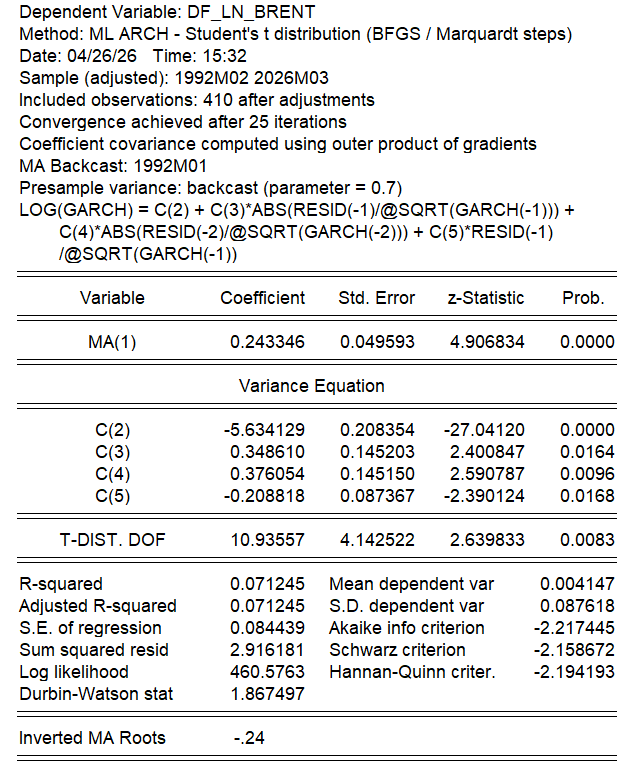
\includegraphics[width=0.8\textwidth]{序列DF_LN_BRENT的MA(1)-EGARCH(2,0)-t模型结果图.png}
\caption{MA(1)-EGARCH(2,0)-t模型结果图（Brent）}
\label{fig:brent_egarch}
\end{figure}

由图~\ref{fig:brent_egarch}可知，序列DF\_LN\_BRENT的MA(1)-EGARCH(2,0)-t模型的均值方程和方差方程为
\begin{align}\label{eq:序列DF_LN_BRENT的MA(1)-EGARCH(2,0)-t模型均值方程}
\mathrm{DF}\_\mathrm{LN}\_\mathrm{BRENT}_t=\varepsilon _t+\theta \varepsilon _{t-1}=\varepsilon _t+0.243346\cdot \varepsilon _{t-1},
\end{align}
\begin{gather}\label{eq:序列DF_LN_BRENT的MA(1)-EGARCH(2,0)-t模型方差方程}
\begin{aligned}
\ln \left( \sigma _{t}^{2} \right) &=\omega +\alpha _1\left| \frac{\varepsilon _{t-1}}{\sigma _{t-1}} \right|+\alpha _2\left| \frac{\varepsilon _{t-2}}{\sigma _{t-2}} \right|+\gamma \left| \frac{\varepsilon _{t-1}}{\sigma _{t-1}} \right|
\\
&= -5.634129+0.348610\left| \frac{\varepsilon _{t-1}}{\sigma _{t-1}} \right|+0.376054\left| \frac{\varepsilon _{t-2}}{\sigma _{t-2}} \right|
\\
&\quad -0.208818\frac{\varepsilon _{t-1}}{\sigma _{t-1}} ,
\end{aligned}
\end{gather}
其中，$\varepsilon_t$ 为扰动项，$\sigma_t^2$ 为条件方差，$\theta$ 为移动平均系数，$\omega$ 为方差方程常数项，$\alpha_1$ 为ARCH项系数(滞后1阶)，$\alpha_2$ 为ARCH项系数(滞后2阶)，$\gamma$ 为非对称项系数，模型扰动项$\varepsilon _t\sim t(10.93557)$。


\subsubsubsection{Dubai原油价格}\hspace{0pt}\par

\vspace{6pt}

DF\_LN\_DUBAI序列的GARCH族模型优选结果见表~\ref{tab:dubai_garch_p}和表~\ref{tab:dubai_garch_criteria}。

\begin{table}[H]
\centering
\caption{DF\_LN\_DUBAI序列GARCH族模型系数显著性检验结果}
\label{tab:dubai_garch_p}
\setlength{\tabcolsep}{4pt}  % 适当缩小列间距以适应页面
\begin{tabular}{lccccc}
\toprule[1.2pt]
\multirow{2}{*}{$\quad\quad\,\,\,\,\,$模型名称} & \multicolumn{4}{c}{系数显著性(p值)}  \\
\cmidrule(lr){2-5}
& 常数项C & ARCH项 & 非对称项 & GARCH项 \\
\midrule[0.75pt]
AR(1)-GARCH(1,0)-t     & 0.0000 & 0.0876 & - & - \\
AR(1)-GARCH(2,0)-t     & 0.0000 & 0.2283 / 0.2437 & - & - \\
AR(1)-GARCH(1,1)-t     & 0.1577 & 0.3083 & - & 0.6335 \\
AR(1)-GARCH(1,2)-t     & 0.0444 & 0.1967 & - & 0.1310 / 0.1013 \\
AR(1)-GARCH(2,1)-t     & 0.6293 & 0.3454 / 0.9815 & - & 0.8787 \\
AR(1)-GARCH(2,2)-t     & 0.0009 & 0.1269 / 0.1441 & - & 0.9455 / 0.2267 \\
\midrule
AR(1)-TARCH(1,0)-t     & 0.0000 & 0.2956 & 0.0063 & - \\
AR(1)-TARCH(2,0)-t     & 0.0000 & 0.3888 / 0.5015 & 0.0076 & - \\
AR(1)-TARCH(1,1)-t     & 0.0000 & 0.5026 & 0.0068 & 0.5418 \\
AR(1)-TARCH(1,2)-t     & 0.0001 & 0.5900 & 0.0057 & 0.6664 / 0.7452 \\
AR(1)-TARCH(2,1)-t     & 0.0000 & 0.5036 / 0.9671 & 0.0072 & 0.6278 \\
AR(1)-TARCH(2,2)-t     & 0.0000 & 0.5998 / 0.0964 & 0.0065 & 0.2366 / 0.9086 \\
\midrule
AR(1)-EGARCH(1,0)-t    & \textbf{0.0000} & \textbf{0.0013} & \textbf{0.0101} & - \\
AR(1)-EGARCH(2,0)-t    & \textbf{0.0000} & \textbf{0.0015} / \textbf{0.0137} & \textbf{0.0166} & - \\
AR(1)-EGARCH(1,1)-t    & \textbf{0.0118} & \textbf{0.0099} & \textbf{0.0218} & \textbf{0.0000} \\
AR(1)-EGARCH(1,2)-t    & 0.0205 & 0.0101 & 0.0171 & 0.0610 / 0.1884 \\
AR(1)-EGARCH(2,1)-t    & 0.0338 & 0.0183 / 0.7554 & 0.0175 & 0.0003 \\
AR(1)-EGARCH(2,2)-t    & 0.0390 & 0.0131 / 0.4136 & 0.0146 & 0.4972 / 0.0789 \\
\bottomrule[1.2pt]
\end{tabular}
\end{table}

\begin{table}[H]
\centering
\caption{DF\_LN\_DUBAI序列GARCH族模型信息准则结果对比}
\label{tab:dubai_garch_criteria}
\setlength{\tabcolsep}{4pt}  % 适当缩小列间距以适应页面
\begin{tabular}{lcccc}
\toprule[1.2pt]
\multirow{2}{*}{$\quad\quad\,\,\,\,\,$模型名称} & \multicolumn{1}{c}{p值} & \multicolumn{3}{c}{信息准则} \\
\cmidrule(lr){2-2} \cmidrule(lr){3-5}
& MA(1) & AIC & SC & HQ \\
\midrule[0.75pt]
AR(1)-GARCH(1,0)-t     & 0.0000 & -2.150568 & -2.111314 & -2.135037 \\
AR(1)-GARCH(2,0)-t     & 0.0001 & -2.127236 & -2.078168 & -2.107822 \\
AR(1)-GARCH(1,1)-t     & 0.0003 & -2.044434 & -1.995366 & -2.025020 \\
AR(1)-GARCH(1,2)-t     & 0.0000 & -2.085860 & -2.026979 & -2.062563 \\
AR(1)-GARCH(2,1)-t     & 0.0018 & -2.046218 & -1.987337 & -2.022921 \\
AR(1)-GARCH(2,2)-t     & 0.0000 & -2.193008 & -2.124314 & -2.165828 \\
\midrule
AR(1)-TARCH(1,0)-t     & 0.0000 & -2.310822 & -2.261755 & -2.291408 \\
AR(1)-TARCH(2,0)-t     & 0.0000 & -2.308010 & -2.249129 & -2.284713 \\
AR(1)-TARCH(1,1)-t     & 0.0000 & -2.308616 & -2.249735 & -2.285319 \\
AR(1)-TARCH(1,2)-t     & 0.0000 & -2.304437 & -2.235743 & -2.277257 \\
AR(1)-TARCH(2,1)-t     & 0.0000 & -2.303728 & -2.235034 & -2.276548 \\
AR(1)-TARCH(2,2)-t     & 0.0000 & -2.304617 & -2.226109 & -2.273554 \\
\midrule
AR(1)-EGARCH(1,0)-t    & 0.0000 & -2.273970 & -2.224903 & -2.254556 \\
AR(1)-EGARCH(2,0)-t    & 0.0000 & -2.284499 & -2.225618 & -2.261202 \\
AR(1)-EGARCH(1,1)-t    & 0.0000 & \textbf{-2.296263} & \textbf{-2.237382} & \textbf{-2.272965} \\
AR(1)-EGARCH(1,2)-t    & 0.0000 & -2.294569 & -2.225875 & -2.267389 \\
AR(1)-EGARCH(2,1)-t    & 0.0000 & -2.291505 & -2.222811 & -2.264325 \\
AR(1)-EGARCH(2,2)-t    & 0.0000 & -2.292254 & -2.213746 & -2.261191 \\
\bottomrule[1.2pt]
\end{tabular}
\end{table}

由表~\ref{tab:dubai_garch_p}和表~\ref{tab:dubai_garch_criteria}可知，最优模型为AR(1)-EGARCH(1,1)-t，所有系数显著且信息准则表现最优。其结果如图\ref{fig:dubai_egarch}所示。

\begin{figure}[H]
\centering
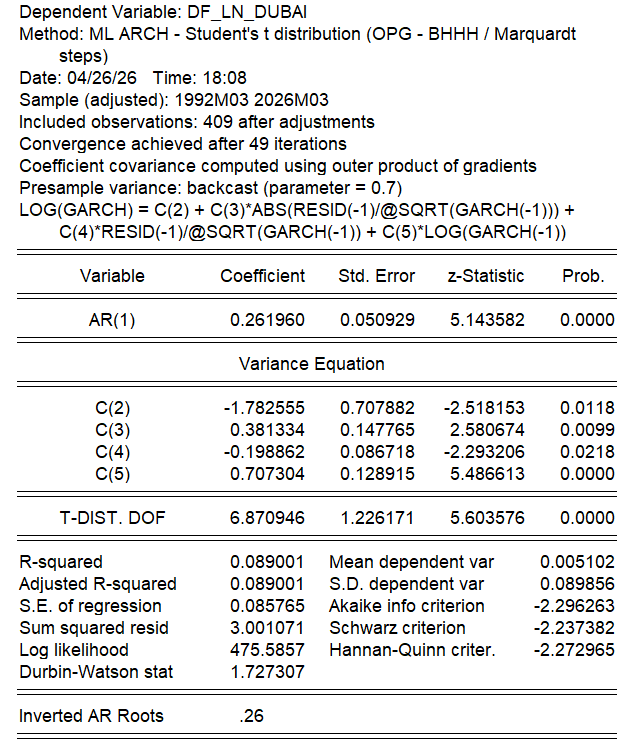
\includegraphics[width=0.8\textwidth]{序列DF_LN_DUBAI的MA(1)-EGARCH(1,1)模型结果图.png}
\caption{AR(1)-EGARCH(1,1)-t模型结果图（Dubai）}
\label{fig:dubai_egarch}
\end{figure}

由图~\ref{fig:dubai_egarch}可知，序列DF\_LN\_DUBAI的AR(1)-EGARCH(1,1)-t模型的均值方程和方差方程为
\begin{gather}\label{eq:序列DF_LN_DUBAI的MA(1)-EGARCH(1,1)-t模型均值方程}
\begin{aligned}
\mathrm{DF}\_\mathrm{LN}\_\mathrm{DUBAI}_t&=\phi \cdot \mathrm{DF}\_\mathrm{LN}\_\mathrm{DUBAI}_{t-1}+\varepsilon _t
\\
&=0.261960\cdot \mathrm{DF}\_\mathrm{LN}\_\mathrm{DUBAI}_{t-1}+\varepsilon _t,
\end{aligned}
\end{gather}
\begin{gather}\label{eq:序列DF_LN_DUBAI的MA(1)-EGARCH(1,1)-t模型方差方程}
\begin{aligned}
\ln \left( \sigma _{t}^{2} \right) &=\omega +\alpha \left| \frac{\varepsilon _{t-1}}{\sigma _{t-1}} \right|+\gamma \frac{\varepsilon _{t-1}}{\sigma _{t-1}}+\beta \ln \left( \sigma _{t-1}^{2} \right) 
\\
&=-1.782555+ 0.381334\cdot \left| \frac{\varepsilon _{t-1}}{\sigma _{t-1}} \right|-0.198862\cdot \frac{\varepsilon _{t-1}}{\sigma _{t-1}}
\\
&\quad + 0.707304\cdot \ln \left( \sigma _{t-1}^{2} \right) ,
\end{aligned}
\end{gather}
其中，$\varepsilon_t$ 为扰动项，$\sigma_t^2$ 为条件方差，$\phi$ 为自回归系数，$\omega$ 为方差方程常数项，$\alpha$ 为ARCH项系数，$\gamma$ 为非对称项系数，$\beta$ 为GARCH项系数，模型扰动项$\varepsilon _t\sim t(6.870946)$。


\subsubsection{残差白噪声检验}

对各序列的最优GARCH族模型的残差序列做Q检验，结果分别如图~\ref{fig:序列DF_LN_WTI的MA(1)-EGARCH(1,1)模型残差的Q检验结果图}、图~\ref{fig:MA(1)-EGARCH(2,0)-t模型的残差白噪声检验结果图(Brent)}、图~\ref{fig:MA(1)-EGARCH(1,1)-t模型的残差白噪声检验结果图(Dubai)}所示。
\begin{figure}[H]
\centering
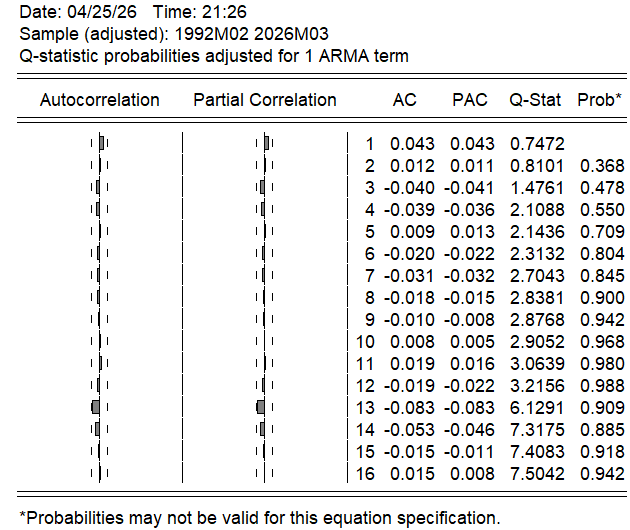
\includegraphics[width=0.7\textwidth]{序列DF_LN_WTI的MA(1)-EGARCH(1,1)模型残差的Q检验结果图.png}
\caption{MA(1)-EGARCH(1,1)-t模型的残差白噪声Q检验结果图（WTI）}
\label{fig:序列DF_LN_WTI的MA(1)-EGARCH(1,1)模型残差的Q检验结果图}
\end{figure}

\begin{figure}[H]
\centering
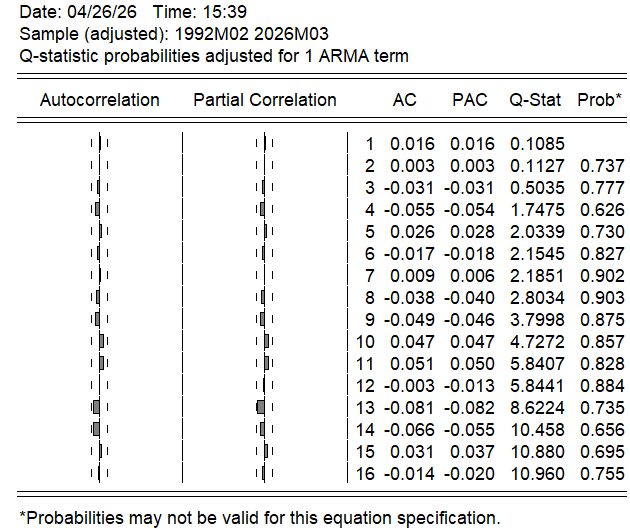
\includegraphics[width=0.8\textwidth]{MA(1)-EGARCH(2,0)-t模型的残差白噪声检验结果图.png}
\caption{MA(1)-EGARCH(2,0)-t模型的残差白噪声Q检验结果图（Brent）}
\label{fig:MA(1)-EGARCH(2,0)-t模型的残差白噪声检验结果图(Brent)}
\end{figure}

\begin{figure}[H]
\centering
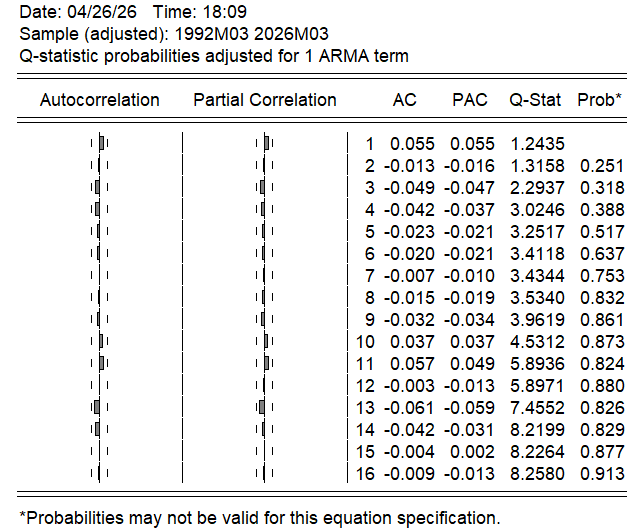
\includegraphics[width=0.8\textwidth]{MA(1)-EGARCH(1,1)-t模型的残差白噪声检验结果图.png}
\caption{AR(1)-EGARCH(1,1)-t模型的残差白噪声Q检验结果图（Dubai）}
\label{fig:MA(1)-EGARCH(1,1)-t模型的残差白噪声检验结果图(Dubai)}
\end{figure}

由图~\ref{fig:序列DF_LN_WTI的MA(1)-EGARCH(1,1)模型残差的Q检验结果图}、图~\ref{fig:MA(1)-EGARCH(2,0)-t模型的残差白噪声检验结果图(Brent)}、图~\ref{fig:MA(1)-EGARCH(1,1)-t模型的残差白噪声检验结果图(Dubai)}可知，各滞后阶数的Q统计量伴随概率均大于0.05的显著性水平，无法拒绝残差序列为白噪声的原假设。表明三个最优GARCH族模型均已充分提取序列的均值与波动信息，残差无自相关，模型设定合理。




\subsubsection{条件异方差检验}

对三个序列的最优GARCH族模型残差序列分别做滞后4、5、6阶的ARCH-LM检验，结果见表~\ref{tab:ARCH-LM1111}。

\begin{table}[H]
\centering
\caption{三个序列的最优GARCH族模型残差的ARCH-LM检验p值}
\label{tab:ARCH-LM1111}
\setlength{\tabcolsep}{4pt}  % 适当缩小列间距以适应页面
\begin{tabular}{lcccc ccc}
\toprule[1.2pt]
\multirow{2}{*}{$\quad\quad\quad\quad\,\,\,\,\,\,\,\,$序列(模型)} & \multicolumn{3}{c}{F统计量p值}  \\
\cmidrule(lr){2-4}
& 滞后4阶 & 滞后5阶 & 滞后6阶 \\
\midrule[0.75pt]
DF\_LN\_WTI(MA(1)-EGARCH(1,1)-t)   & 0.3148 & 0.4247  & 0.4046  \\
DF\_LN\_BRENT(MA(1)-EGARCH(2,0)-t) & 0.3483 & 0.4782  & 0.5227  \\
DF\_LN\_DUBAI(AR(1)-EGARCH(1,1)-t) & 0.9107 & 0.9570  & 0.9243  \\
\bottomrule
\end{tabular}
\end{table}

根据表~\ref{tab:ARCH-LM1111}可知，三个模型的滞后4、5、6阶的p值均大于0.05，这说明这三个模型均已充分捕捉原序列的条件异方差。

对三个序列的最优GARCH族模型残差平方序列做Q检验，结果分别见图~\ref{fig:序列DF_LN_WTI的MA(1)-EGARCH(1,1)模型残差平方的Q检验结果图}、图~\ref{fig:序列DF_LN_WTI的MA(1)-EGARCH(1,1)模型残差平方的Q检验结果图11}、图~\ref{fig:序列DF_LN_WTI的MA(1)-EGARCH(1,1)模型残差平方的Q检验结果图21}。

\begin{figure}[H]
\centering
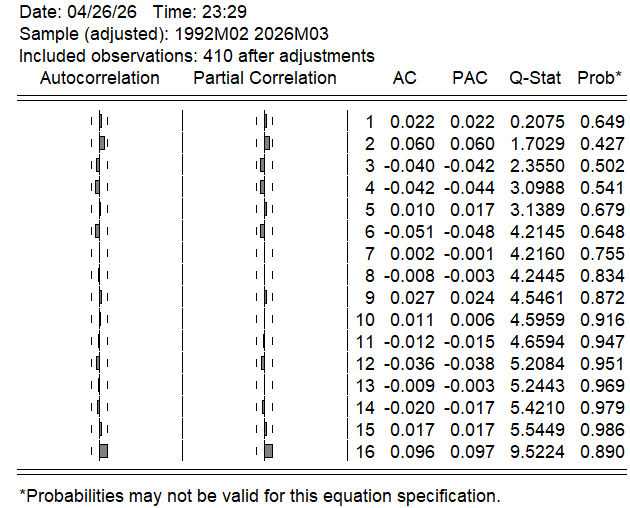
\includegraphics[width=0.8\textwidth]{序列DF_LN_WTI的MA(1)-EGARCH(1,1)模型残差平方的Q检验结果图.png}
\caption{MA(1)-EGARCH(1,1)模型残差平方的Q检验结果图（WTI）}
\label{fig:序列DF_LN_WTI的MA(1)-EGARCH(1,1)模型残差平方的Q检验结果图}
\end{figure}

\begin{figure}[H]
\centering
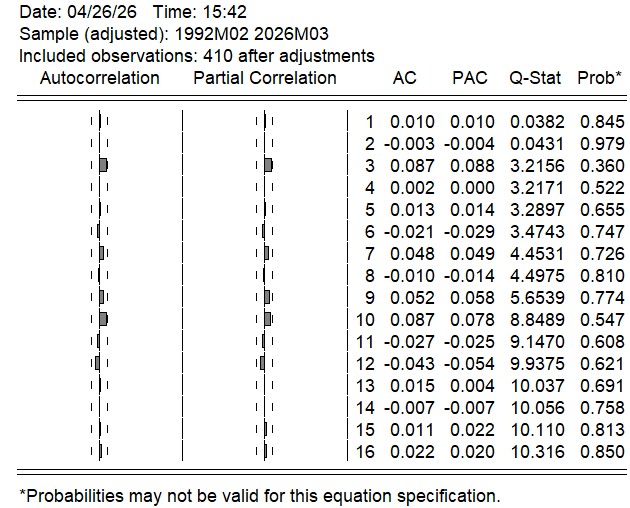
\includegraphics[width=0.8\textwidth]{a(1)-egarch(2,0)-t模型的条件异方差检验结果图4.png}
\caption{MA(1)-EGARCH(2,0)模型残差平方的Q检验结果图（Brent）}
\label{fig:序列DF_LN_WTI的MA(1)-EGARCH(1,1)模型残差平方的Q检验结果图11}
\end{figure}

\begin{figure}[H]
\centering
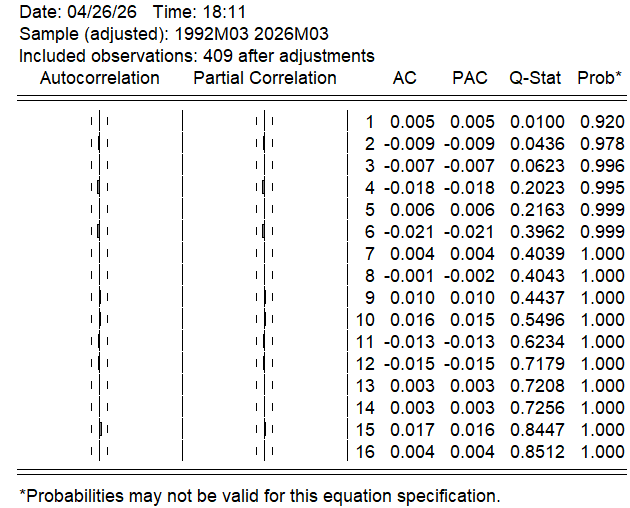
\includegraphics[width=0.8\textwidth]{MA(1)-EGARCH(1,1)-t模型的条件异方差检验结果图4.png}
\caption{AR(1)-EGARCH(1,1)模型残差平方的Q检验结果图（Dubai）}
\label{fig:序列DF_LN_WTI的MA(1)-EGARCH(1,1)模型残差平方的Q检验结果图21}
\end{figure}

由图~\ref{fig:序列DF_LN_WTI的MA(1)-EGARCH(1,1)模型残差平方的Q检验结果图}、图~\ref{fig:序列DF_LN_WTI的MA(1)-EGARCH(1,1)模型残差平方的Q检验结果图11}、图~\ref{fig:序列DF_LN_WTI的MA(1)-EGARCH(1,1)模型残差平方的Q检验结果图21}可知，这三个模型各滞后期的p值均大于0.05，表明残差序列不存在显著自相关。

综上可知，这三个最优GARCH族模型均已充分捕捉原序列的条件异方差。


\newpage
\section{模型结果分析}

为深入分析三大国际原油价格市场的波动特征差异，本文在最优均值方程的基础上，分别构建了GARCH族模型，并基于Student's \(t\)分布捕捉收益率的尖峰厚尾特征。表~\ref{tab:final_params} 汇总了三大原油价格最优GARCH模型的核心参数估计结果。

\begin{table}[H]
\centering
\caption{三大原油价格最优GARCH模型核心参数对比}
\label{tab:final_params}
\begin{tabular}{lcccccc}
\toprule
原油品种 & 均值模型 & 均值系数 & ARCH项（\(\alpha\)） & 杠杆项（\(\gamma\)） & GARCH项（\(\beta\)） \\
\midrule
WTI   & MA(1) & 0.2272 & 0.2974   & -0.1621 & 0.7972 \\
Brent & MA(1) & 0.2433 & 0.3486 / 0.3761 & -0.2088 & --- \\
Dubai & AR(1) & 0.2620 & 0.3813   & -0.1989 & 0.7073 \\
\bottomrule
\end{tabular}
\end{table}

\subsection{均值方程分析}

根据表~\ref{tab:final_params}可知，三大原油的对数收益率序列均表现出显著的\textbf{一阶短期记忆特征}。WTI和Brent采用MA(1)模型，表明当期收益率受上一期新息（冲击）的正向影响；Dubai采用AR(1)模型，表明其收益率受上一期自身收益率的影响更显著。从均值系数来看，Dubai（0.2620）> Brent（0.2433）> WTI（0.2272），说明Dubai市场的短期价格惯性最强。这一特征反映了亚太地区对中东原油的高度依赖，其现货主导的定价机制缺乏成熟期货市场的价格平滑与套期保值功能，导致价格对自身历史值的依赖更为显著。

\subsection{波动方程分析}

\subsubsection{ARCH项（\(\alpha\)）：短期冲击的敏感性}

ARCH项反映了新信息对当期波动的直接影响。Dubai的ARCH系数最大（0.3813），表明其\textbf{对地缘政治、供应中断等突发冲击的反应最为敏感}。WTI的ARCH系数为0.2974，Brent的两期ARCH系数分别为0.3486和0.3761，表明Brent对连续冲击的响应更为持久。这一结果与Dubai原油以现货定价为主、缺乏成熟期货对冲机制的现实高度一致。

\subsubsection{杠杆项（\(\gamma\)）：非对称性}

三大原油的杠杆项系数均为负且统计显著，验证了原油市场普遍存在\textbf{杠杆效应}，即存在负向冲击对波动的放大作用强于正向冲击的非对称特征。其中：
\begin{itemize}
\item Brent的杠杆效应最强（\(\gamma = -0.2088\)），反映其作为全球定价基准，对负面消息（如地缘冲突、需求骤降）反应最为剧烈；
\item Dubai次之（\(\gamma = -0.1989\)），WTI最弱（\(\gamma = -0.1621\)），说明WTI市场受结构性因素（如管道运输、库存）影响更大，价格弹性相对较低。
\end{itemize}

\subsubsection{GARCH项（\(\beta\)）：波动持续性}

GARCH项衡量冲击对波动的影响持续时间。WTI的GARCH系数高达0.7972，接近1，表明其\textbf{波动衰减最慢}，一次冲击的影响可长期存在。这与其区域市场特征相符，WTI交割地为库欣（美国俄克拉荷马州的一个小镇，全球最重要的原油交割中心之一），易受管道运输、库存等结构性瓶颈制约。Dubai的GARCH系数为0.7073，持续性也较强。相比之下，Brent模型中未包含GARCH项（即\(\beta=0\)），表明其波动仅依赖ARCH项，\textbf{冲击衰减最快}，符合其作为全球流动性最高、信息效率最高的市场特征。

\subsection{综合对比与市场解释}

将三大原油市场的波动特征差异归纳为表~\ref{tab:comparison}。

\begin{table}[H]
\centering
\caption{三大原油市场波动特征综合对比}
\label{tab:comparison}
\begin{tabular}{lccc}
\toprule
市场特征 & WTI & Brent & Dubai \\
\midrule
波动持续性 & 最强（\(\beta=0.7972\)） & 无GARCH项，衰减快 & 中等（\(\beta=0.7073\)） \\
短期冲击敏感度 & 中等（\(\alpha=0.2974\)） & 强（双期ARCH） & 最强（\(\alpha=0.3813\)） \\
杠杆效应强度 & 弱（\(\gamma=-0.1621\)） & 最强（\(\gamma=-0.2088\)） & 中等（\(\gamma=-0.1989\)） \\
市场主导特征 & 结构性制约 & 信息效率高 & 供应冲击敏感 \\
\bottomrule
\end{tabular}
\end{table}

综上，三大原油市场的波动特征差异本质上源于其定价机制、交易结构和市场功能的不同。\textbf{Brent是全球最活跃的金融定价基准，信息反应最快；WTI受实物交割瓶颈制约，波动持久；Dubai代表亚太进口市场，对现货冲击最敏感}。


\newpage
\section{结论}

本文基于1992年1月至2026年3月的月度价格数据，运用ARMA-EGARCH模型对WTI、Brent和Dubai三大国际原油市场的对数收益率序列进行了系统的波动建模与对比分析。主要结论如下：

\begin{enumerate}
\item \textbf{序列特征与模型设定}：三大原油原始价格序列均为非平稳过程，一阶差分后平稳且存在显著的条件异方差和尖峰厚尾特征。最优均值模型分别为WTI和Brent的MA(1)以及Dubai的AR(1)，表明原油市场具有短期可预测性。采用Student's \(t\)分布的EGARCH模型能够有效拟合其尾部风险。

\item \textbf{杠杆效应普遍存在}：三大原油市场均表现出显著的波动非对称性，负向冲击对价格波动的放大作用强于同幅度正向冲击。其中，Brent的杠杆效应最强（\(\gamma=-0.2088\)），反映其作为全球基准对负面信息的敏感性最高。

\item \textbf{波动持续性差异显著}：
\begin{itemize}
\item \textbf{WTI} 的GARCH系数最高（\(\beta=0.7972\)），波动衰减最慢，受北美区域管道运输、库存等结构性因素制约；
\item \textbf{Brent} 无GARCH项，冲击衰减仅依赖ARCH项，波动持续性最低，信息效率最高；
\item \textbf{Dubai} 的ARCH项最大（\(\alpha=0.3813\)），对短期冲击最敏感，符合亚太市场对中东原油供应中断的脆弱性。
\end{itemize}

\item \textbf{实际意义与研究价值}：本研究验证了EGARCH-\(t\)模型在能源商品波动建模中的适用性，揭示了三大基准原油在波动传导机制上的本质差异，为投资者、风险管理者和政策制定者提供了量化依据。\textbf{Brent适合短期对冲策略，WTI需关注长期波动风险，Dubai则需防范突发供应冲击}。

\item \textbf{研究局限与展望}：本文采用月度数据，未来可引入日度或高频数据以捕捉更精细的波动特征；此外，可进一步引入外生变量（如地缘政治风险指数、美元指数、库存变化）构建扩展GARCH模型，探讨波动传导机制的外部驱动因素。
\end{enumerate}





% 参考文献

\nocite{*}% 显示所有参考文献（原本只显示已引用的参考文献）
\printbibliography[title={参考文献}]










\end{document}